\chapter{Methods}\label{ch:methods}
\section{Modelling work}
\subsection{Behavioral analysis}\label{sec:behavioral analysis}
% misschien nog handig:
% The magnitude of these forces represents the magnitude of the forces which can be expected for the tree frog and are calculated using the Equations visible in Equations \ref{eq:static_equilibrium_normal} and \ref{eq:static_equilibrium_tang}. The parameters used for the frog weight and the surface area of the adhesive pads are derived from a study by Langowski et al. In this study, tree frogs of the species \textit{Hyla cinerea} were evaluated. The mass of these frogs was $ 6.2e-3 – 8.2e-3 [kg]$ and the adhesive pads of these frogs measured $0.45 [mm]$ in height, $1 [mm]$ in width and $1.5 [mm]$ in length \cite{langowski2018force}. The total adhesive surface area $A_{tot}$ for the tree frog is calculated with Equation \ref{eq:surface_area} with $N = 18$ for the number of toes of the frog and $R_{toe} = 0.6 [mm]$ for the radius of the toe with is assumed circular. Using these parameters, the shear force has a value of $F_{t = 3.37e3 [N/m^2]}$ and the normal force has a value of $F_n = 3.75e2 [N/m^2]$. 

\qquad In Section \ref{sec:intro_spreading} is described how tree frogs spread their legs when an increase in adhesional performance is required. This section further evaluates the impact of this spreading on the forces at the contact interface.\\

\qquad The forces acting on the epithelial layer of the adhesive pad can be decomposed in normal forces and tangential forces. These forces are respectively perpendicular and tangential to the surface the frog is adhered to. The magnitude of the forces that act on the tree frog are determined by the position of the frog and the weight of the frog. For a frog that is sitting on a vertical wall a schematic representation of the forces is visible is Figure \ref{fig:tree_frog_with_forces}. The adhesive pads of the tree frog are thus subjected to tangential ($F_{t,1}, F_{t,2}$) and normal ($F_{n,1}, F_{n,2}$) forces. The normal forces are for the largest part determined by the weight and the posture of the frog while the tangential forces can be increased by the frog by proximal pulling of the adhesive pads over the surface. The direction of the normal force in the attachment point I is opposed to the direction of the normal force in point II. A schematic representation of the situation is visible in the free body diagram in Figure \ref{fig:FBD_2D}.\\ 

\begin{figure}[h]
\begin{subfigure}{0.24\textwidth}
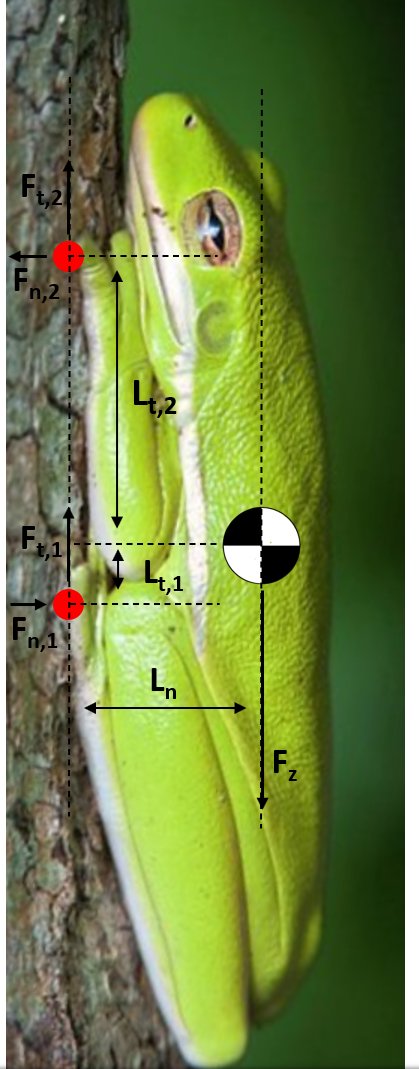
\includegraphics[width=4cm, height=8cm,angle=0]{images/limb spreading/tree_frog_forces_vertical.PNG}
\caption{}
\label{fig:tree_frog_with_forces}
\end{subfigure}
\hspace{0.8in}
\begin{subfigure}{0.24\textwidth}
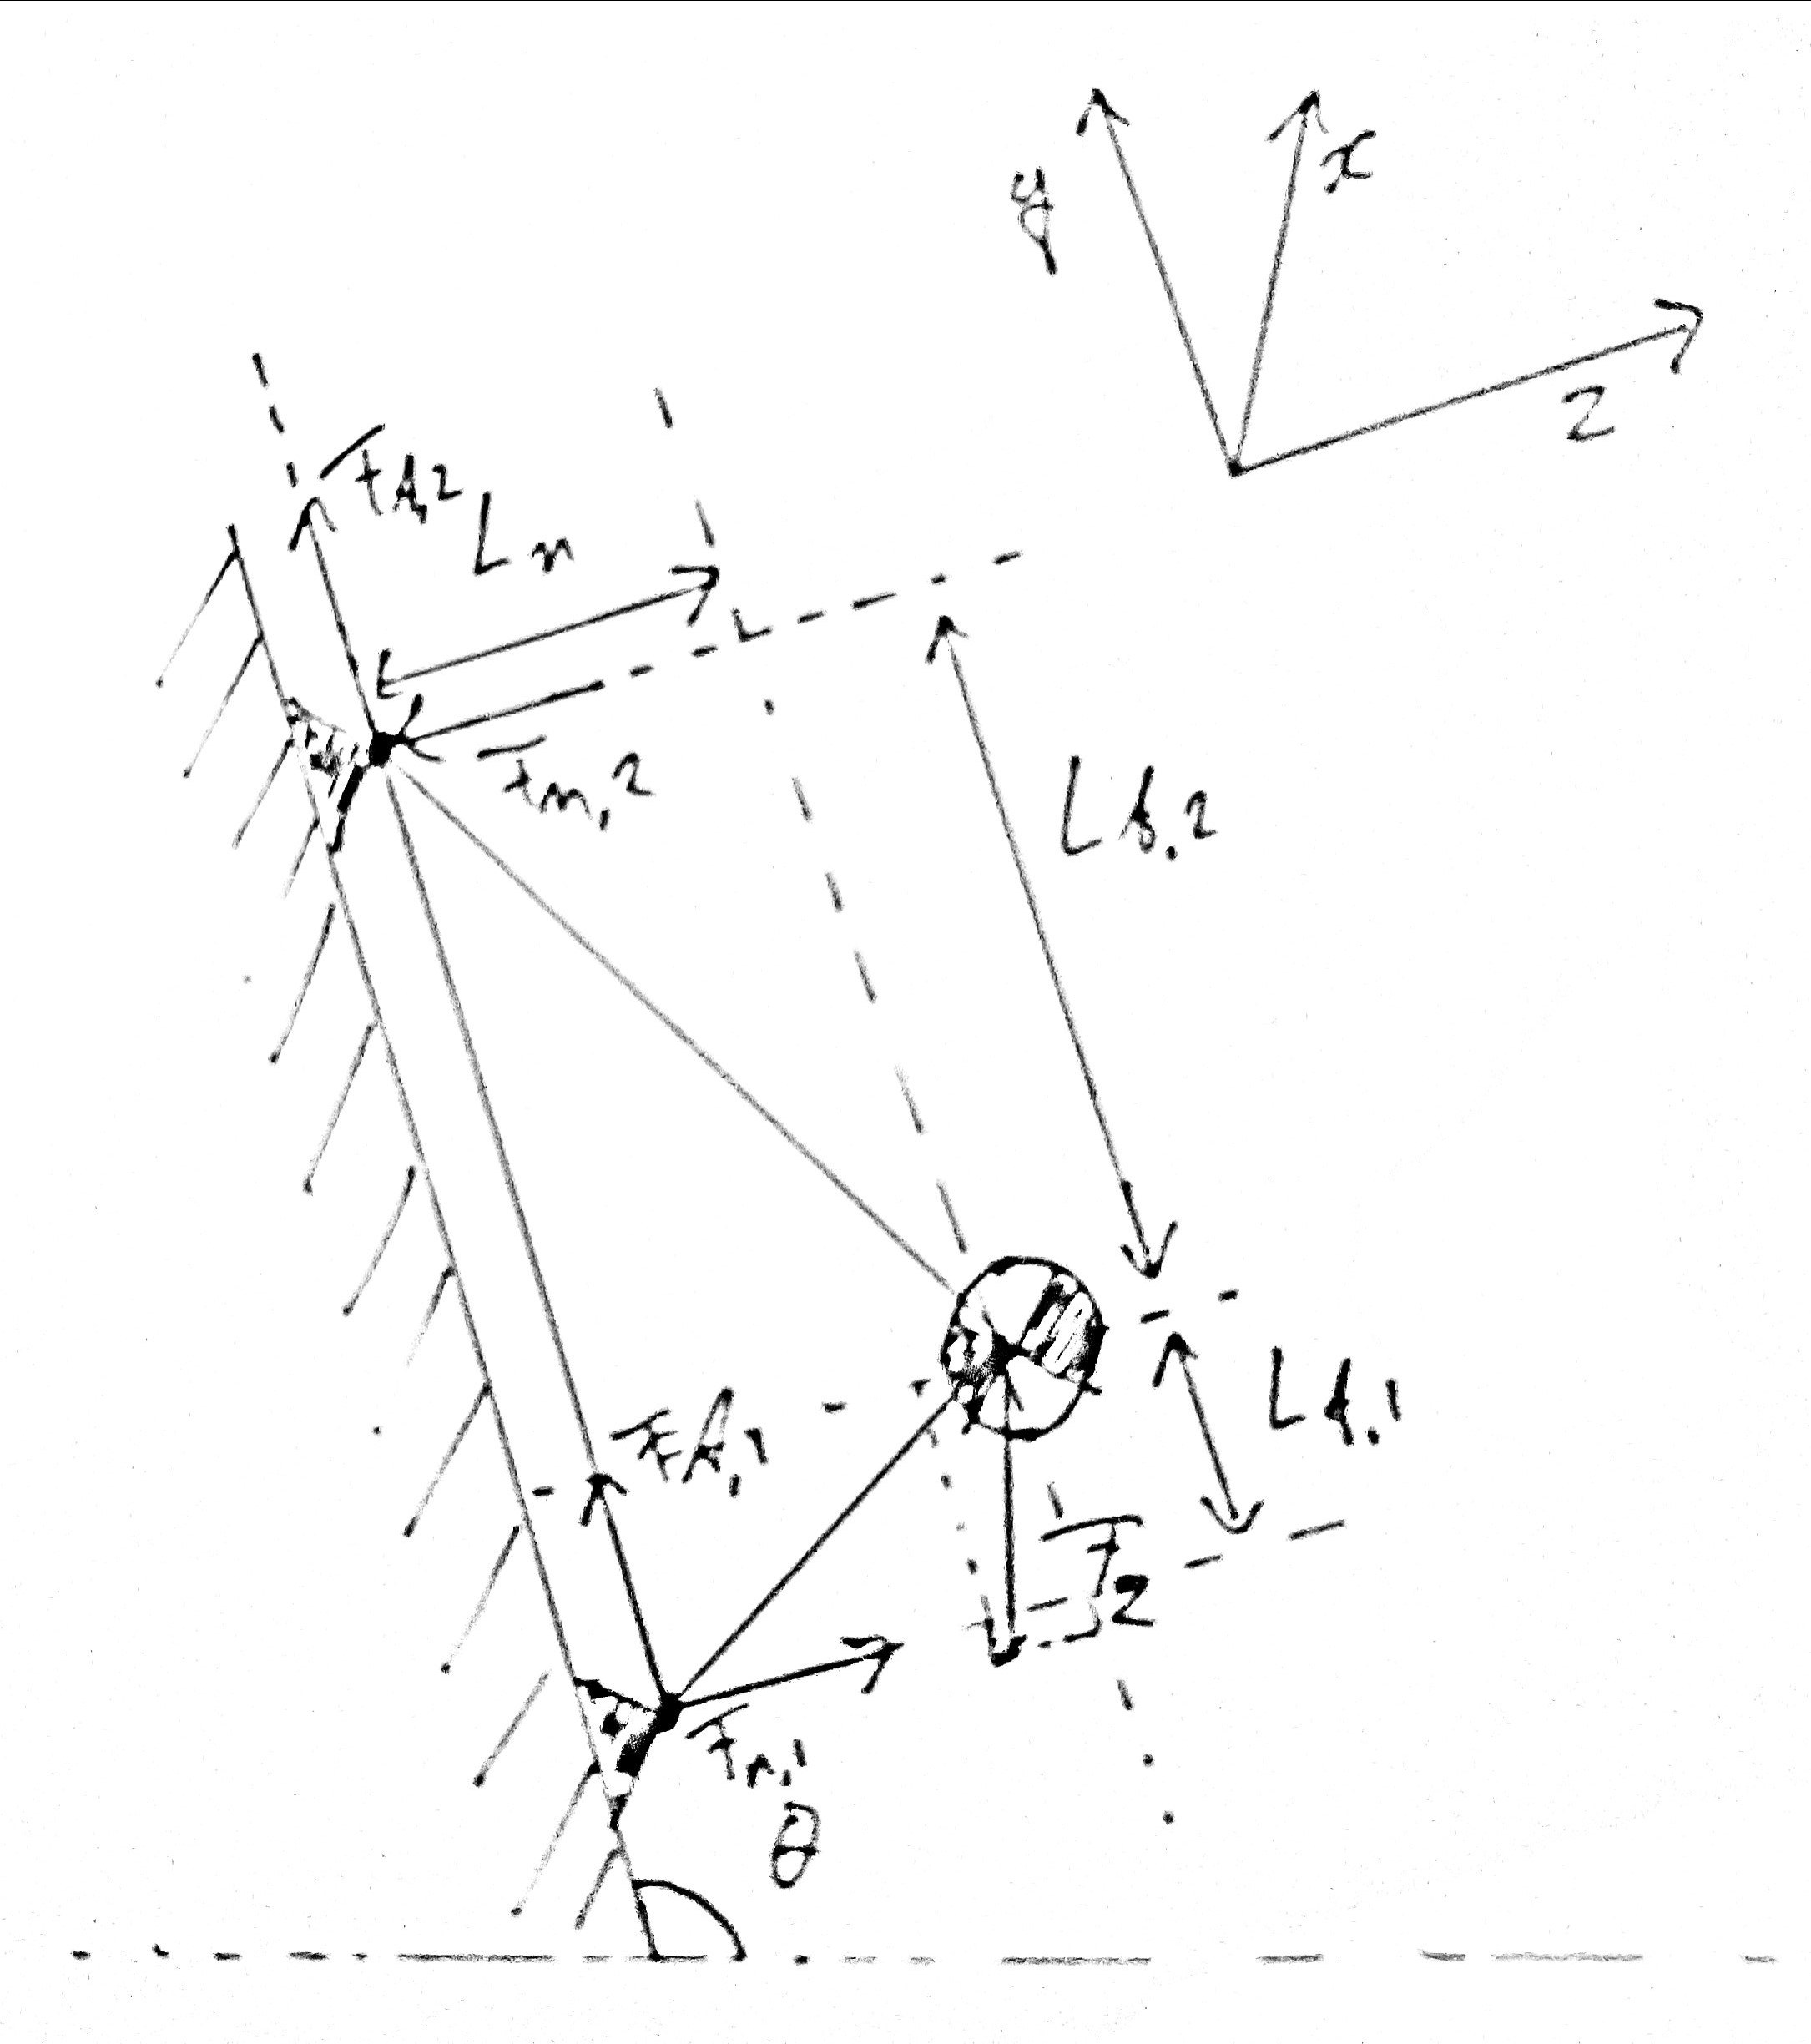
\includegraphics[width=5cm, height=8cm, angle=0]{images/limb spreading/FBD_frog_angle.jpg}
\caption{}
\label{fig:FBD_2D}
\end{subfigure}
\caption{Forces on a tree frog in resting position with in (a) the Hyla Cinerea with the relevant forces and dimensions and in (b) the free body diagram of the same situation}
\label{fig:FBD_tree_frog}
\end{figure}

\qquad The normal forces acting on the limbs of the frog can be fully defined using static equilibrium equations. The tangential forces however, can not be easily determined because the problem is statically over constrained and thus static indeterminate. Typically, such problems can be solved when the mechanical properties of the rigid body are known. The mechanical properties of the body of the tree frog connecting the two attachment points are dependent on the tree frog and can therefore not be easily determined. Furthermore, the tangential forces can be manipulated by the frog itself. The frog can create a force between the limbs with the application of a proximal pull. This proximal pulling is also described in Section \ref{sec:intro_spreading} and is visible in Figure \ref{fig:limb_spreading_rest}-\ref{fig:limb_spreading_second_spread}. The behaviour visible is displayed by the frog when the surface the frog is sitting on, is rotated so that the frog needs a larger adhesional force in order to prevent falling off.\\ 

\qquad The forces at the surface of the adhesive pads are visible in Figure \ref{fig:frog_feet}. The proximal pulling forces $F_{p,1}$ and $F_{p,2}$ are oriented towards the center of gravity and can be decomposed in the x and y-components. 

\begin{figure}[h!]
    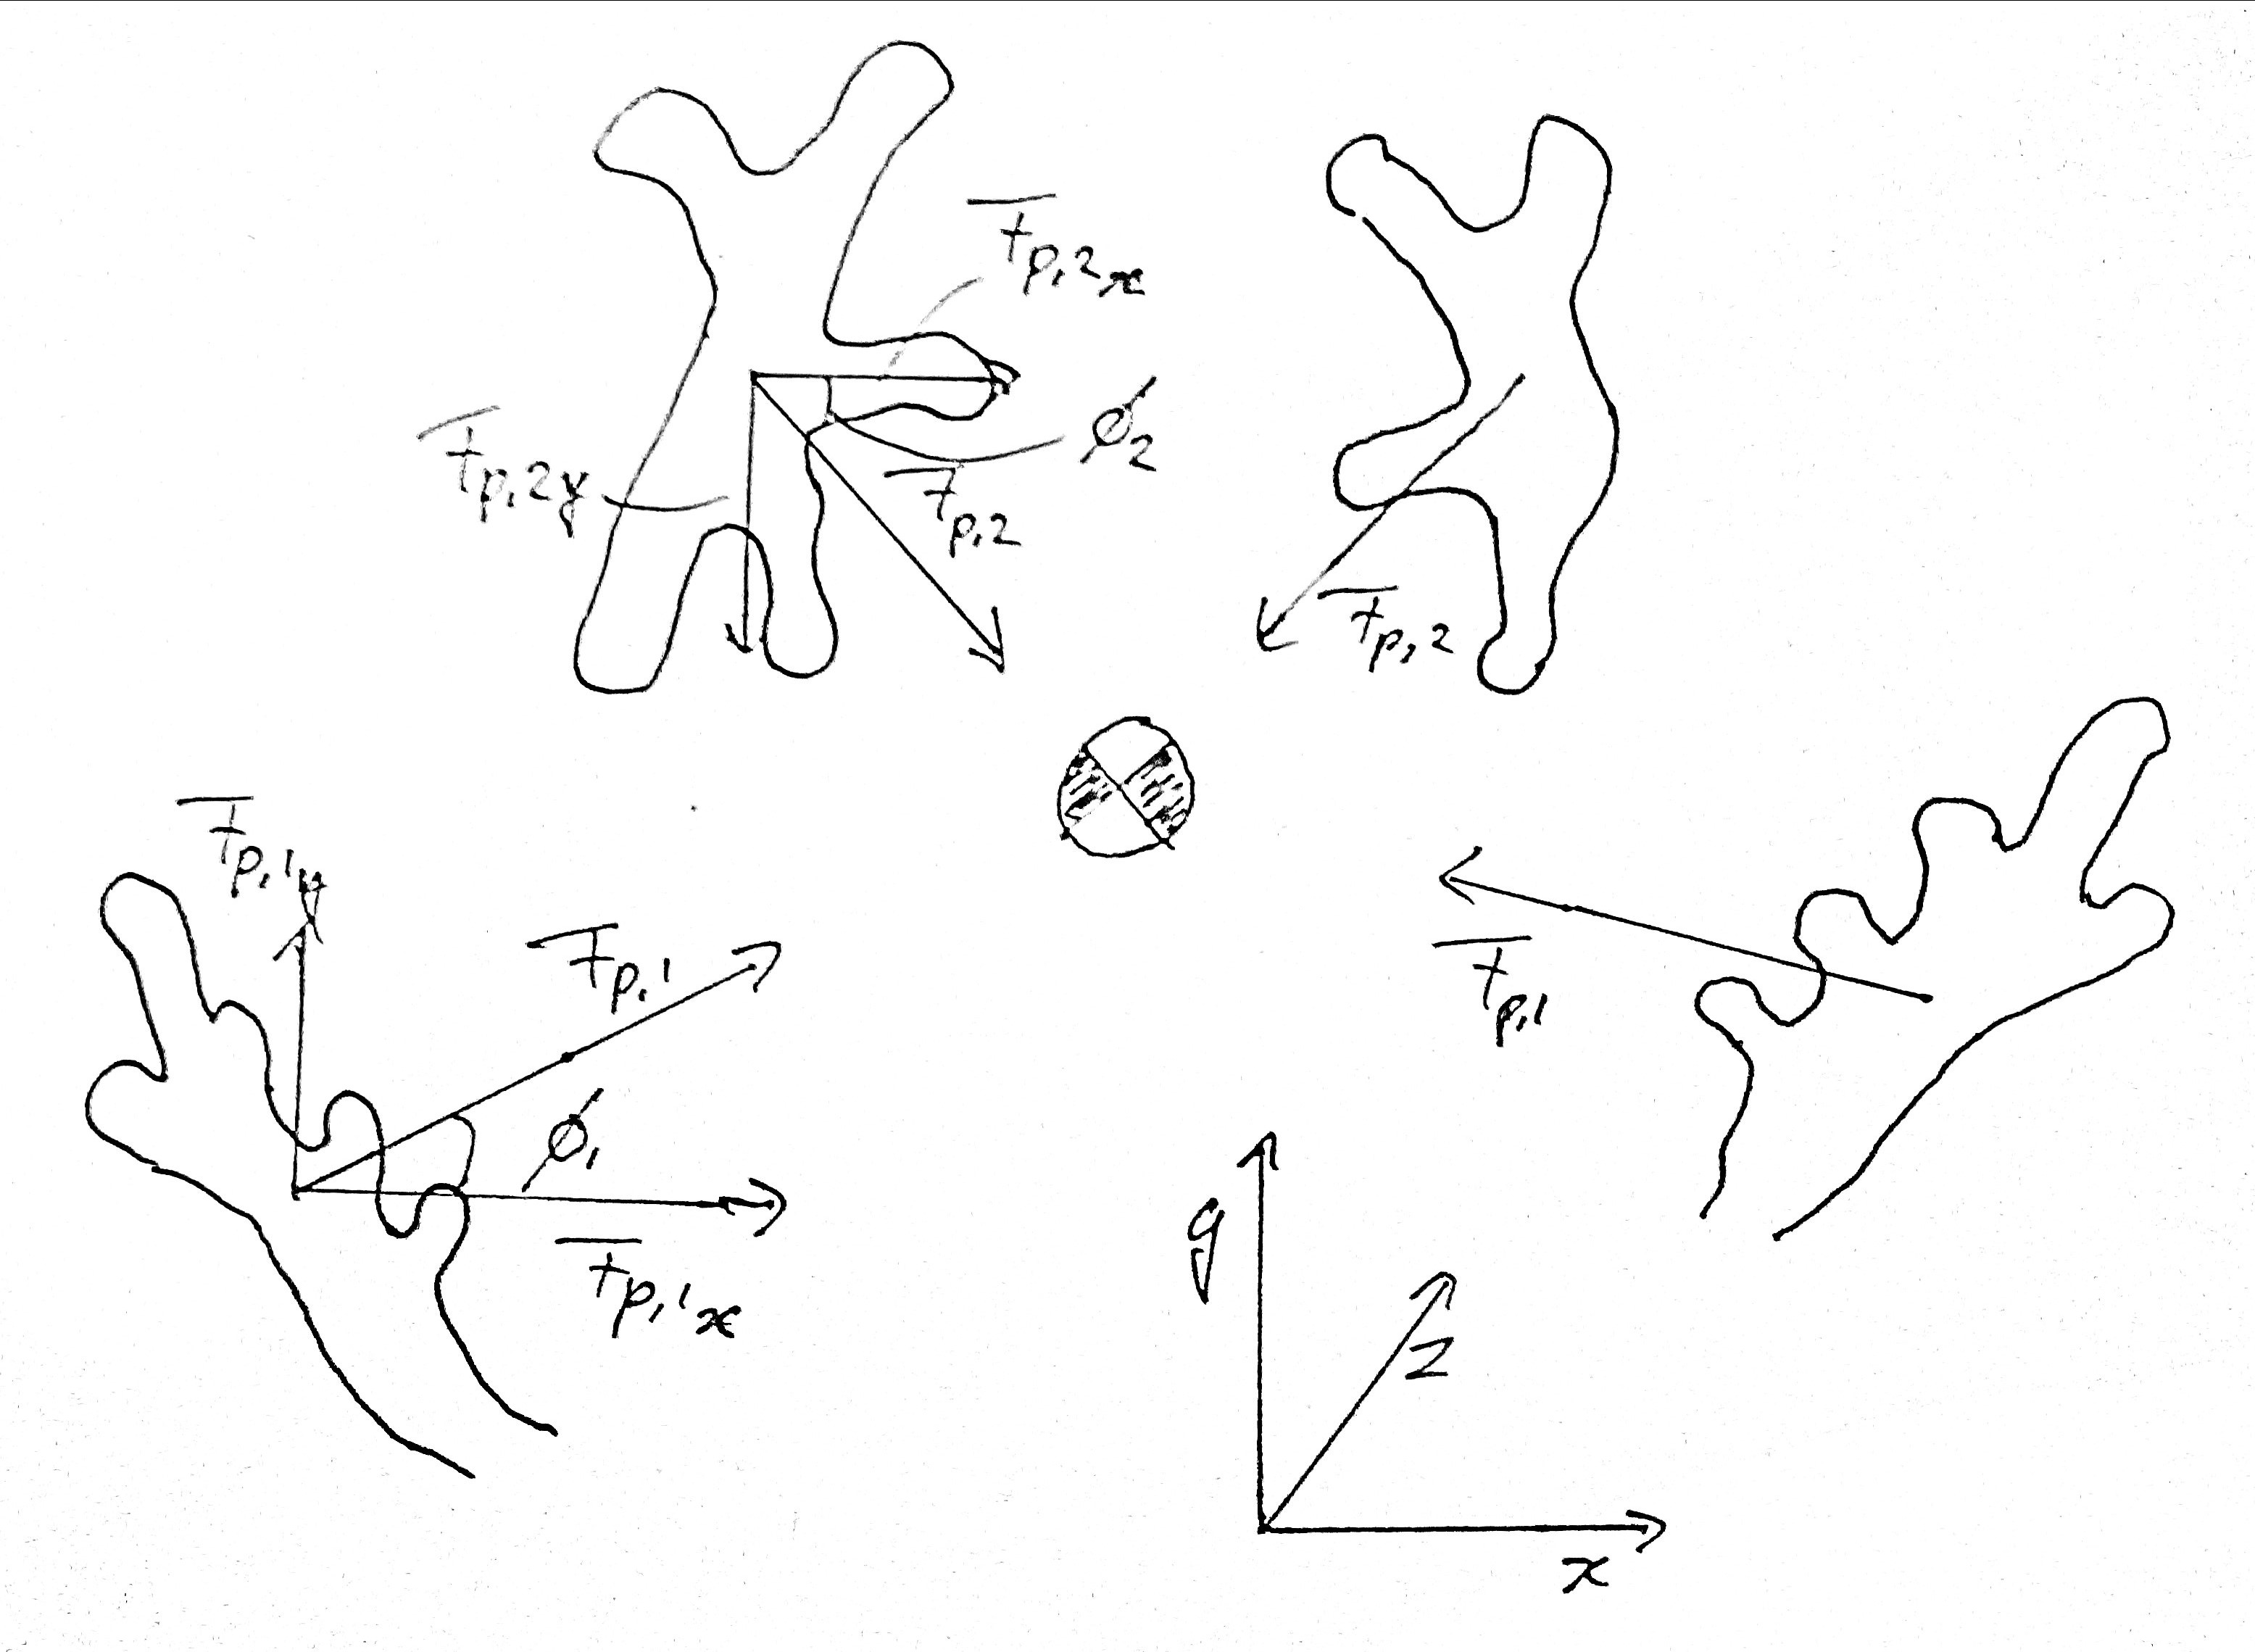
\includegraphics[width=0.65\linewidth, height=7cm, angle=0]{images/limb spreading/frog_feet_streched.jpg}
    \caption{The adhesive surfaces on the frog feet seen from below. The proximal pulling forces $F_{p,1}$ and $F_{p,2}$ are decomposed in force components in the x-direction as $F_{p,1_x}$ and $F_{p,2_x}$. The force components in the y-direction are represented by $F_{p,1_y}$ and $F_{p,2_y}$.}
    \label{fig:frog_feet}
\end{figure}

\qquad The limb spreading does also influence the angles of attachment $\alpha_{1}$ and $\alpha_{2}$ as visible in Figure \ref{fig:frog_schematic}. The tangential forces on the adhesive surfaces of the frog are split up in a component representing the proximal pulling $F_{p}$ and in components representing the rest of the tangential force on the adhesive surfaces, $F_{s,1}$ and $F_{s,2}$. The magnitude of $F_{s,1}$ and $F_{s,2}$ is unknown because the FBD of the frog is statically indeterminate and we do not known the stiffness properties of the frog body connecting the two points of attachment. The relations between these various force components are given by the relations visible in Equation \ref{eq:tangential_forces}.\\ 

\begin{figure}[h!]
    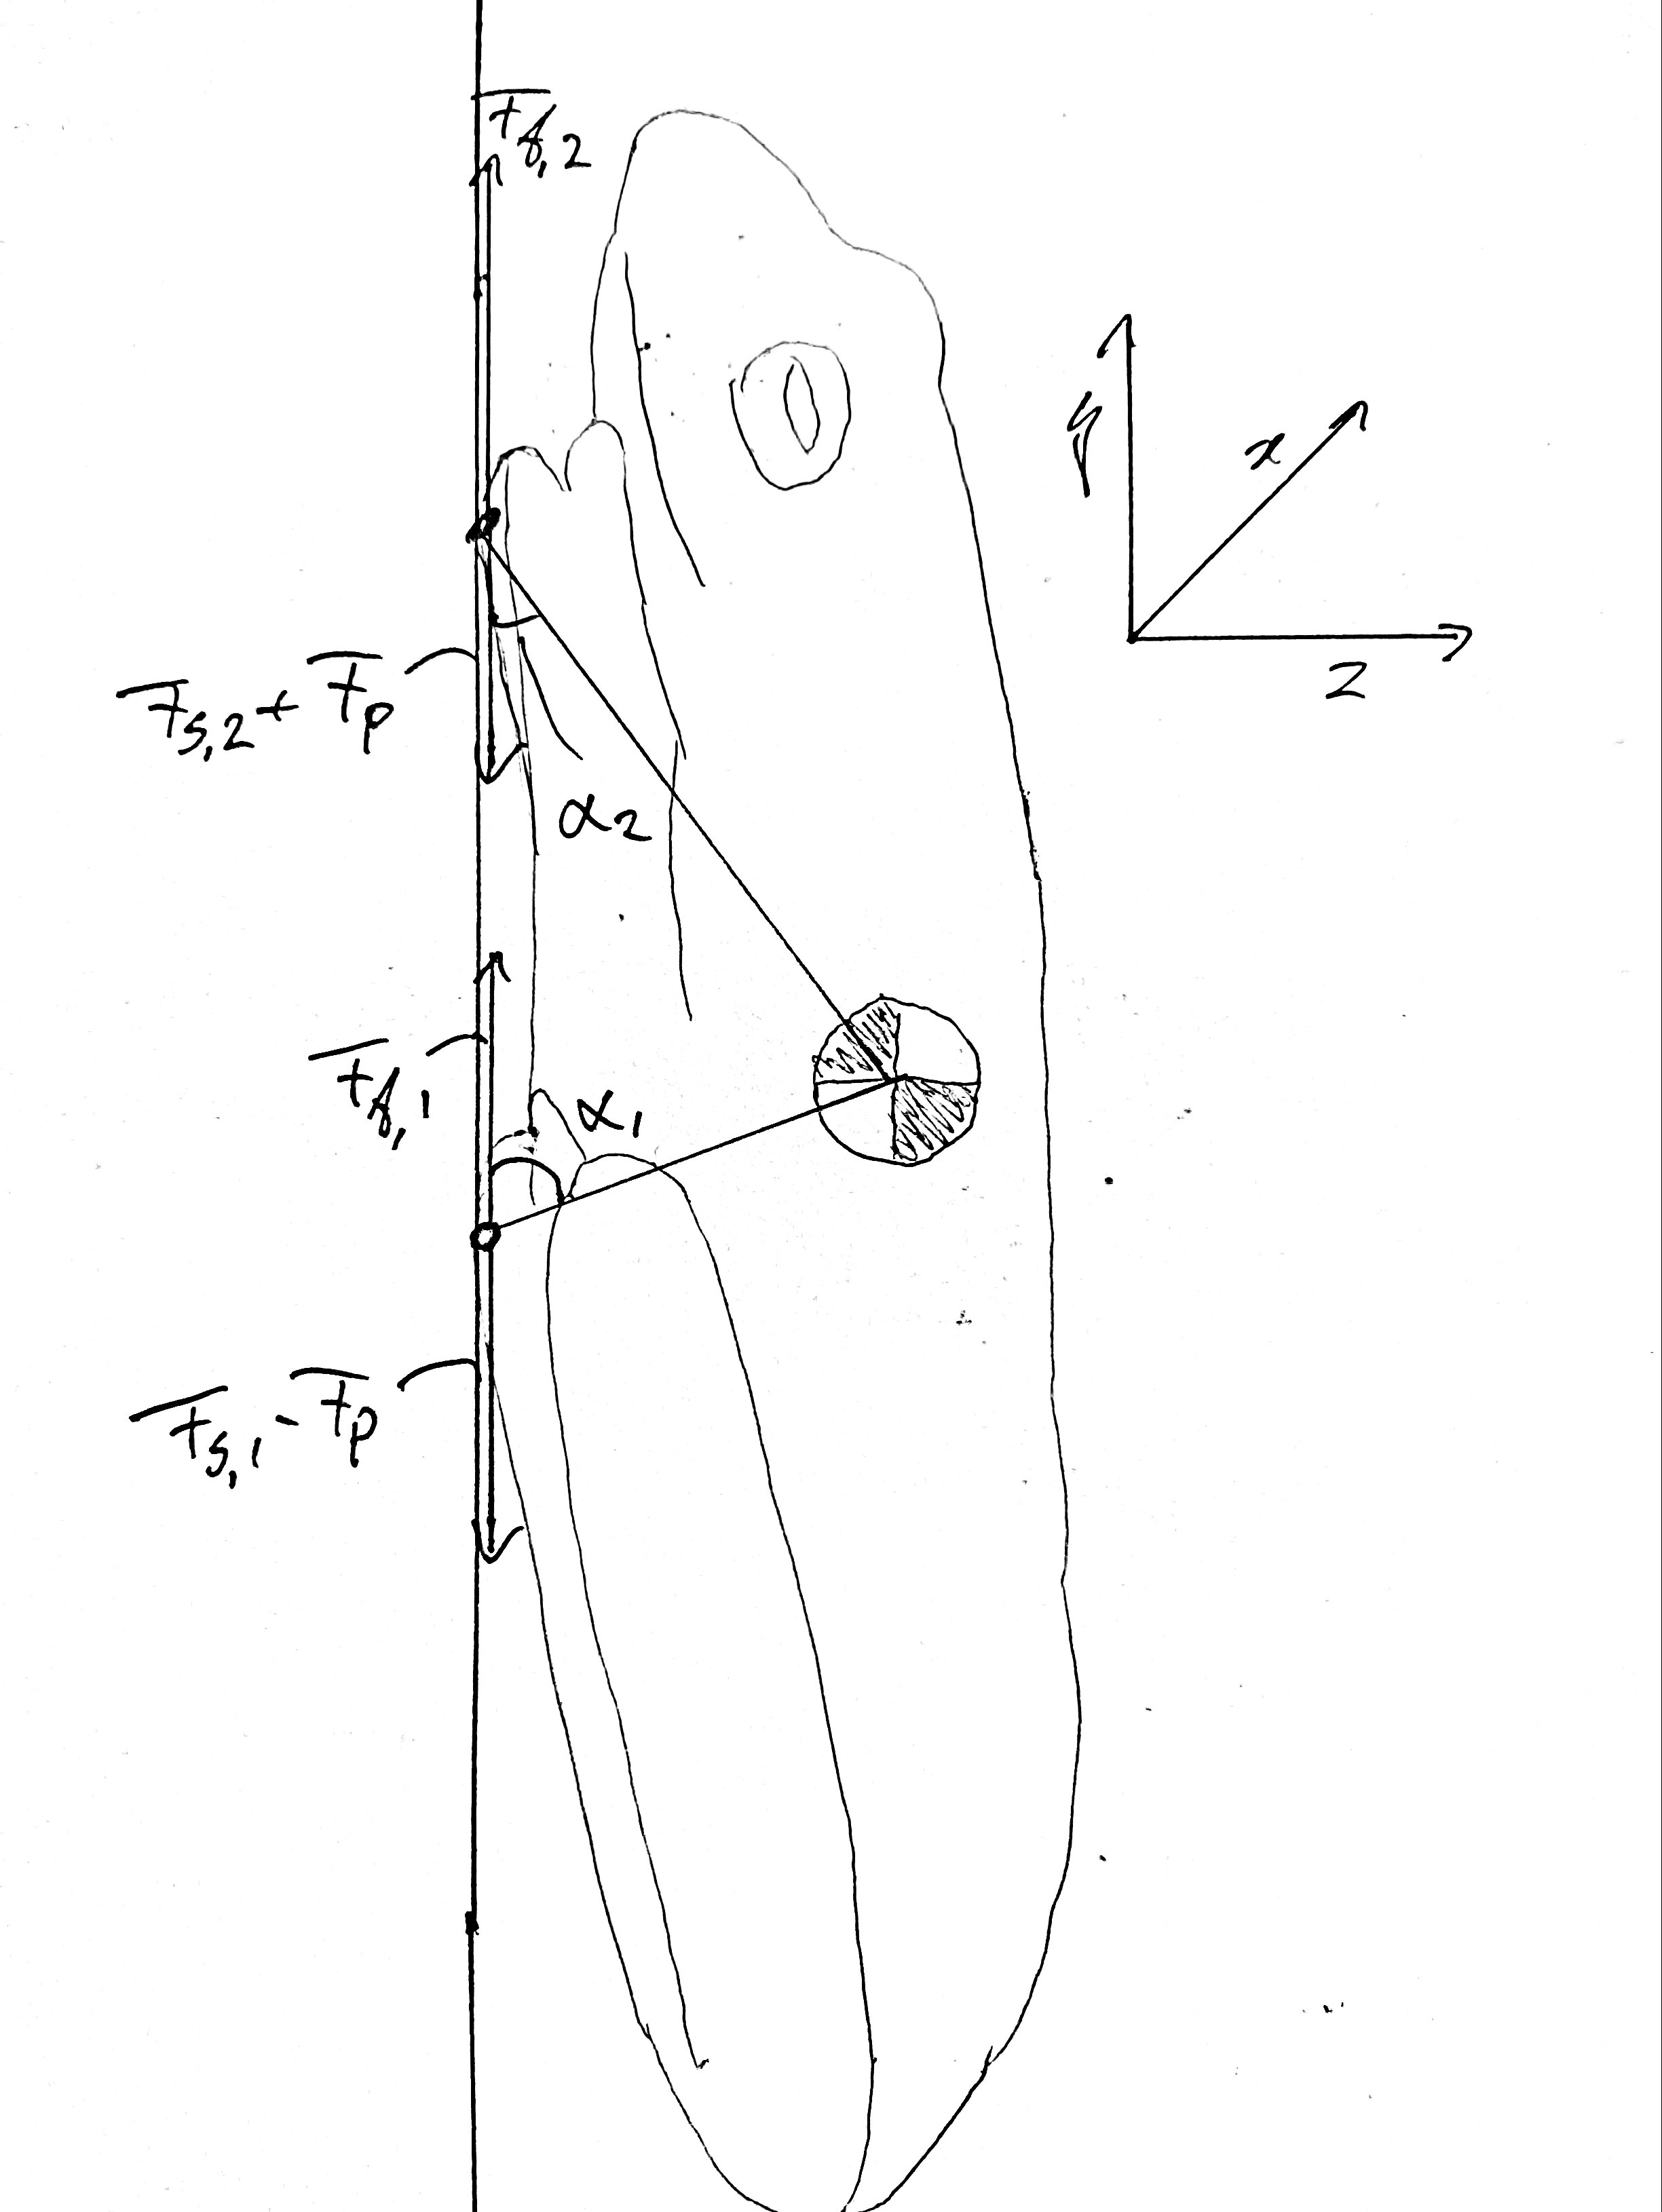
\includegraphics[width=0.55\linewidth, height=7.5cm, angle=0]{images/limb spreading/frog_schematic.jpg}
    \caption{2D side view of the frog adhered to a surface at $\theta = \frac{\pi}{2}$. The angles of attachment are $\alpha_{1}$ and $\alpha_{2} $}
    \label{fig:frog_schematic}
\end{figure}

\begin{gather}
     F_{t,1} = F_{s,1} - F_{p},\nonumber\\[1ex]
     F_{t,2} = F_{s,2} + F_{p},\nonumber\\[1ex]
     F_z = F_{t,1} + F_{t,2}    
     \label{eq:tangential_forces}
\end{gather}

\qquad A Matlab model is written in which three cases are defined. The first case considers a frog that does not make use of proximal pulling. The mechanical properties of the frog body connecting the two points of attachment are assumed as such that the tangential forces are both equal to half of the tangential component of the gravitational force $F_{t,1} = F_{t,2} = \frac{F_{z}}{2} cos(\frac{\pi}{2} - \theta)$. The normal forces are calculated using the relations given in Equation \ref{eq:static_equilibrium_normal}.\\

\begin{gather}
     F_{n,2} = \frac{F_z (L_n cos(\frac{\pi}{2} - \theta) + L_{t,1} cos(\theta))}{L_{t,1} + L_{t,2}},\nonumber\\[1ex]
     F_{n,1} = \frac{F_{z} cos(\frac{\pi}{2} - \theta) L_{n} - L_{t,2} F_{n,2}}{L_{t,1}}
     \label{eq:static_equilibrium_normal}
\end{gather}

\qquad The second case involves a situation in which the frog proximally pulls its limbs. The magnitude of these pulling forces is derived from the work of Endlein et al. \cite{endlein2013sticking} which is also discussed in Section \ref{sec:intro_spreading}. It is assumed that the proximal pulling starts when the frog performs its first spread. The proximal pulling forces increase to their maximal values when the frog performs its second spread. The angles of the first and second spread are taken form the work of Endlein et al. and are $ \theta_1 = 106 [deg]$ and $\theta_2 = 131 [deg]$ respectively. Equations \ref{eq:spreading_forces_0} - \ref{eq:spreading_forces_2} give the magnitudes of the pulling forces as a function of parameter $R$ which resembles the ratio of the body weight of the frog and the magnitude of the pulling force. The value of this parameter is $R = 0.2$ as discussed in Section \ref{sec:intro_spreading}. The parameter $\phi_1$ is the angle of the proximal pulling force as visible in Figure \ref{fig:frog_feet}. 

\begin{gather}
     \text{For } \theta > \theta_{1},\nonumber\\[1ex]
     F_{p,1_x} = F_{p,2_x} = F_{p,1_y} = F_{p,2_y} = 0
     \label{eq:spreading_forces_0}
\end{gather}

\begin{gather}
     \text{For } \theta_{1} \leq \theta \geq \theta_2,\nonumber\\[1ex]
     F_{p,1_x} = F_{p,1_x} = F_z \frac{R}{4},\nonumber\\[1ex]
     F_{p,1_y} = tan(\phi_1)  F_{p,1_x} \quad \text{\&} \quad F_{p,2_y} = tan(\phi_1)  F_{p,2_x}
     \label{eq:spreading_forces_1}
\end{gather}

\begin{gather}
     \text{For } \theta > \theta_2,\nonumber\\[1ex]
     F_{p,1_x} = F_{p,1_x} = F_z R,\nonumber\\[1ex]
     F_{p,1_y} = tan(\phi_1)  F_{p,1_x} \quad \text{\&} \quad F_{p,2_y} = tan(\phi_1)  F_{p,2_x}
     \label{eq:spreading_forces_2}
\end{gather}

\qquad The third cases includes the pulling forces as in case 2 but also includes a positional adjustment of the frog due to the re positioning of the limbs. For $\theta_{1} \leq \theta \geq \theta_2$ the dimensions $L_{t1}\ \&\ L_{t2}$ are multiplied with a factor $\frac{3}{2}$ and parameter $L_{n}$ is multiplied with a factor $\frac{3}{4}$. For the second spread the parameters are multiplied with factors $2$ and $\frac{1}{2}$ for $L_{t1}\ \&\  L_{t2}$ and $L_{n}$ respectively. These values are based on a rough estimate derived from images of the tree frog during its different spreading positions as visible in Figure \ref{fig:tree_frog_limb_spreading}.\\


\qquad The forces involved  for the three cases considered are visible in Figures \ref{fig:case_1}, \ref{fig:case_2} and \ref{fig:case_3}. The normal forces are the same for case 1 and 2 since they are independent of the tangential forces. The tangential forces which are dependent on the proximal pulling are different between case 1 and 2. The value of the tangential components $F_{t,1}$ and $F_{t,2}$ increases with the first spread and with the second spread. The increase of the tangential force components after the first spread is relatively small compared to the increase at the second spread which is proportional to the magnitude of the proximal forces visible in Figure \ref{fig:pulling}. Case 3 shows the forces at the contact interface for a combination of proximal pulling and positional adjustment. It is visible that the tangential components increase as also visible for case 2. The normal force components decrease due to the positional adjustment.\\


\begin{figure}[h!]
    \begin{subfigure}{0.48\textwidth}
    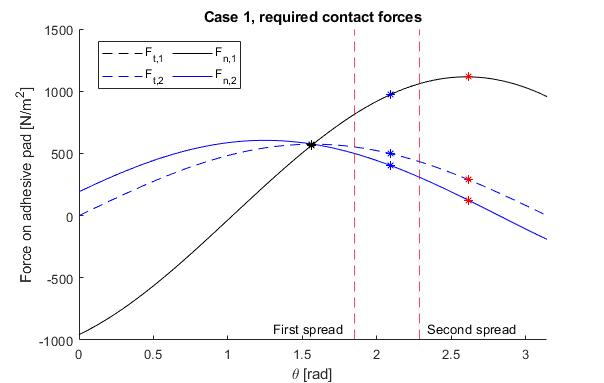
\includegraphics[width=\textwidth, height=5cm, angle=0]{images/limb spreading/FBD_case_1.jpg}
    \caption{}
    \label{fig:case_1}
    \end{subfigure}
    \hfill
    \begin{subfigure}{0.48\textwidth}
    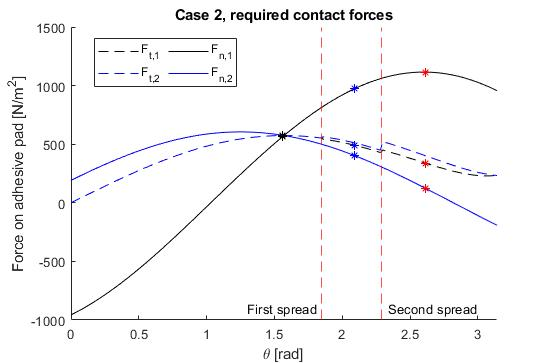
\includegraphics[width=\textwidth, height=5cm, angle=0]{images/limb spreading/FBD_case_2.jpg}
    \caption{}
    \label{fig:case_2}
    \end{subfigure}
    \hfill
    \begin{subfigure}{0.48\textwidth}
    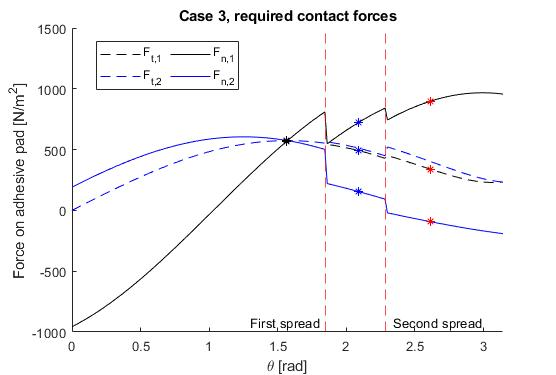
\includegraphics[width=\textwidth, height=5cm, angle=0]{images/limb spreading/FBD_case_3.jpg}
    \caption{}
    \label{fig:case_3}
    \end{subfigure}  
    \begin{subfigure}{0.48\textwidth}
    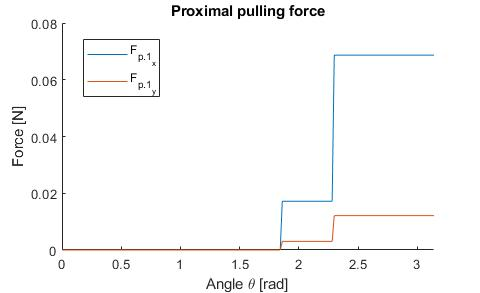
\includegraphics[width=\textwidth, height=5cm, angle=0]{images/limb spreading/pulling_force.jpg}
    \caption{}
    \label{fig:pulling}
    \end{subfigure} 
    \caption{Required contact forces as a function of the the angle $\theta$ for the three cases. The first case in (a) has zero value for every value of $\theta$. In (b), the proximal pulling is included and in (c) positional adjustment is added. The proximal pulling forces for cases 2 and 3 are visible in (d).}
    \label{fig:proximal_pulling_cases}
\end{figure}



\subsection{Discrete fiber model}
\subsubsection{Model fundamentals}\label{sec:discrete_model_fundamentals}
The aim of the discrete fiber model is to replicate the mechanical properties of the epithelial layer by closely mimicking the epithelial geometry and the properties of the various components of the epithelial cell as visible in Figure \ref{fig:epithelial_cell_components}. 


\subsubsection{Model implementation: Geometry}\label{sec:discrete_model_geometry}
The outline of the epithelial cell and its cell components can be seen in Figure \ref{fig:epithelial_cell_components}. The basic outline of the cell and the keratinous part in the the cell are implemented in a 2D model. This model uses  a parameterized Matlab model in which the fibres are proportionally divided over the keratinous domain containing the fibers. This 2D model can be implemented in Solidworks and from Solidworks it can be transferred into Comsol Multiphysics. The Solidworks implementation is visible in Figure \ref{fig:geometry_solidworks}.\\ 

\begin{figure}[h!] 
     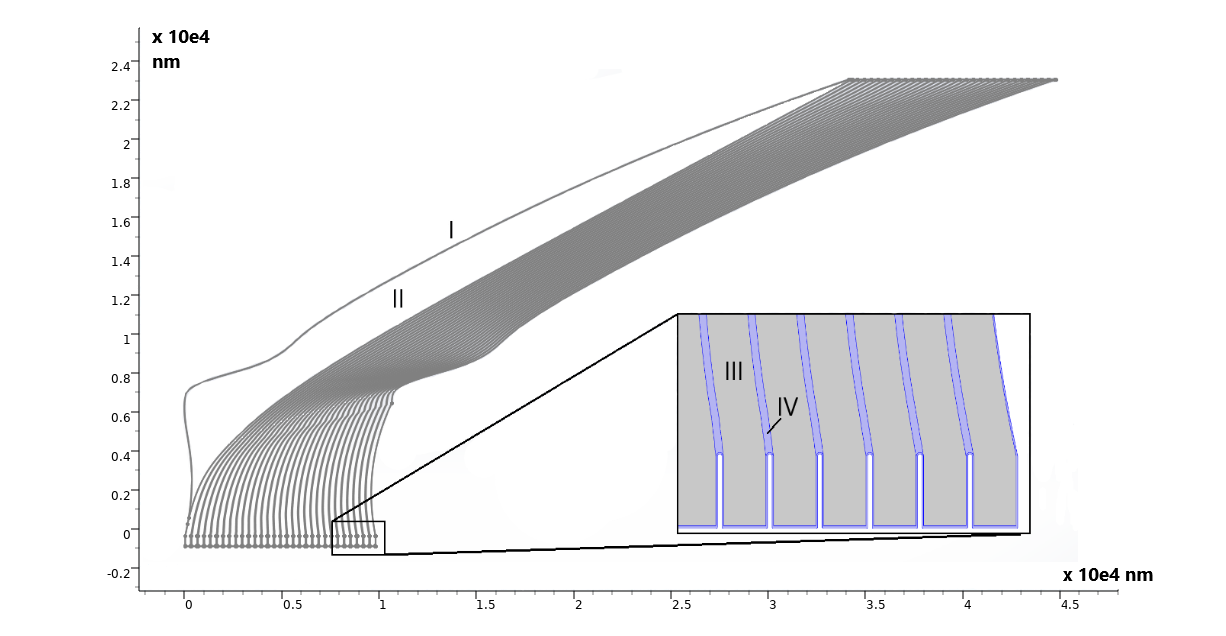
\includegraphics[width=0.85\linewidth, height=6.5cm, angle=0]{images/discrete_model_implementation/solidworks geometry_schematic.png}
     \caption{A representation of the geometry implemented in Solidworks. The keratinous structure is visible in the right part of the cell. The enlarged section shows the individual keratinous fibres. $I$ represents the cornified cell envelope, $II$ the lymph space, $III$ a keratinous fibre and $IV$ the space between the keratinous fibres with forms the matrix in which the fibres are embedded.}
     \label{fig:geometry_solidworks}
\end{figure}

\qquad The geometry visible in Figure \ref{fig:geometry_solidworks} has a relatively high level of complexity due to the presence of the discrete fibers. Comsol Multiphysics needs a mesh in order to perform the finite element analyses. The amount of elements of this mesh increases with the complexity of the geometry and the high level of complexity of the geometry visible in Figure \ref{fig:geometry_solidworks} causes the mesh builder to form a mesh that contains a very large number of mesh elements as visible in Figure \ref{fig:mesh}. The number of mesh elements directly influences the convergence speed of the model. The fiber configuration visible in Figure \ref{fig:geometry_solidworks} however, can be significantly simplified into a rectangular geometry with a reduced number of fibers. The implications of this simplifications are discussed in Section \ref{sec:}.\\

\begin{figure}[h!] 
    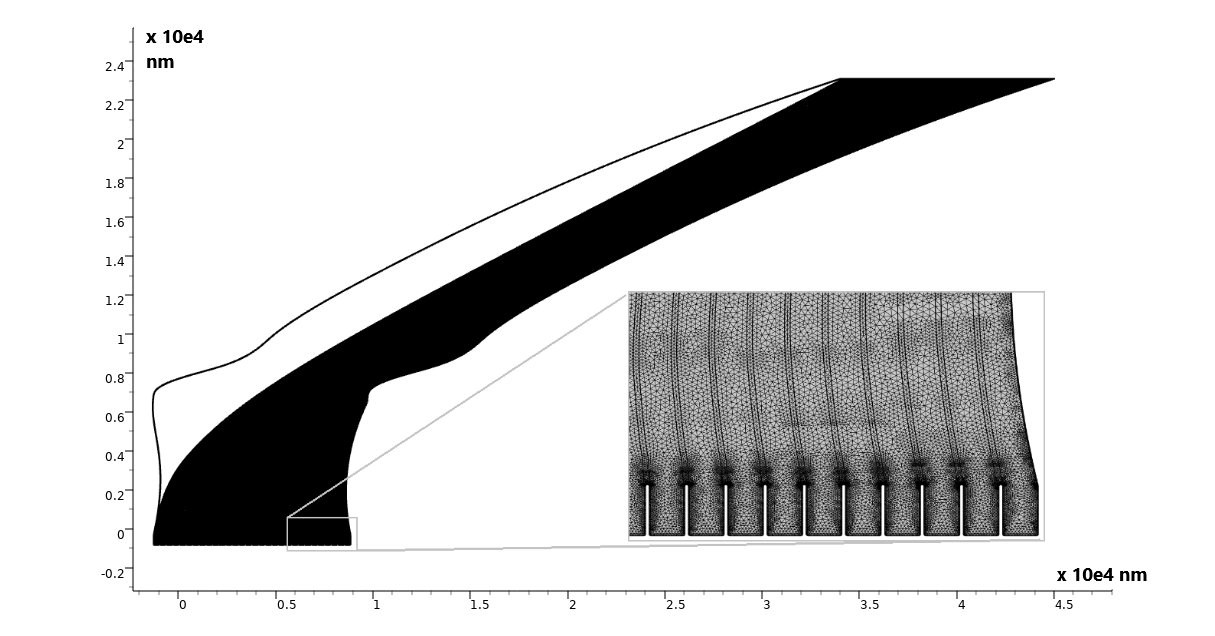
\includegraphics[width=0.85\linewidth, height=6.5cm, angle=0]{images/discrete_model_implementation/mesh_compleet.png}
    \caption{The very dense mesh for the geometry in which one fibre bundle runs from every pillar. This mesh consists of 715790 domain elements and 118113 boundary elements.}
    \label{fig:mesh}
\end{figure}

\qquad The fiber density and the amount of fibers is varied between models to evaluate the consequences of these changes. The standard size of an simplified square fibrous domain is $10\mu m$ in width and $20 \mu m$ in height. This size has the order of magnitude as the size of an epithelial cell. The pillars of the epithelial cell are described to play a role in the establishment of contact between the epithelial layer and the substrate while the channels between the pillars drain excess fluids from the adhesive pads \cite{kappl2016nanoscale}. The pillars however are not described to play a role in the stress distribution along the pad when contact is established and are therefore neglected in the simplified model.


\subsubsection{Model implementation: boundary conditions}\label{sec:discrete_model_boundary_con}
The boundary conditions used in the model resemble the mechanical properties of the epithelial cell layer of the tree frog and need to such that the model is loaded in a similar way as an epithelial cell.\\ 

\begin{figure}[h!] 
    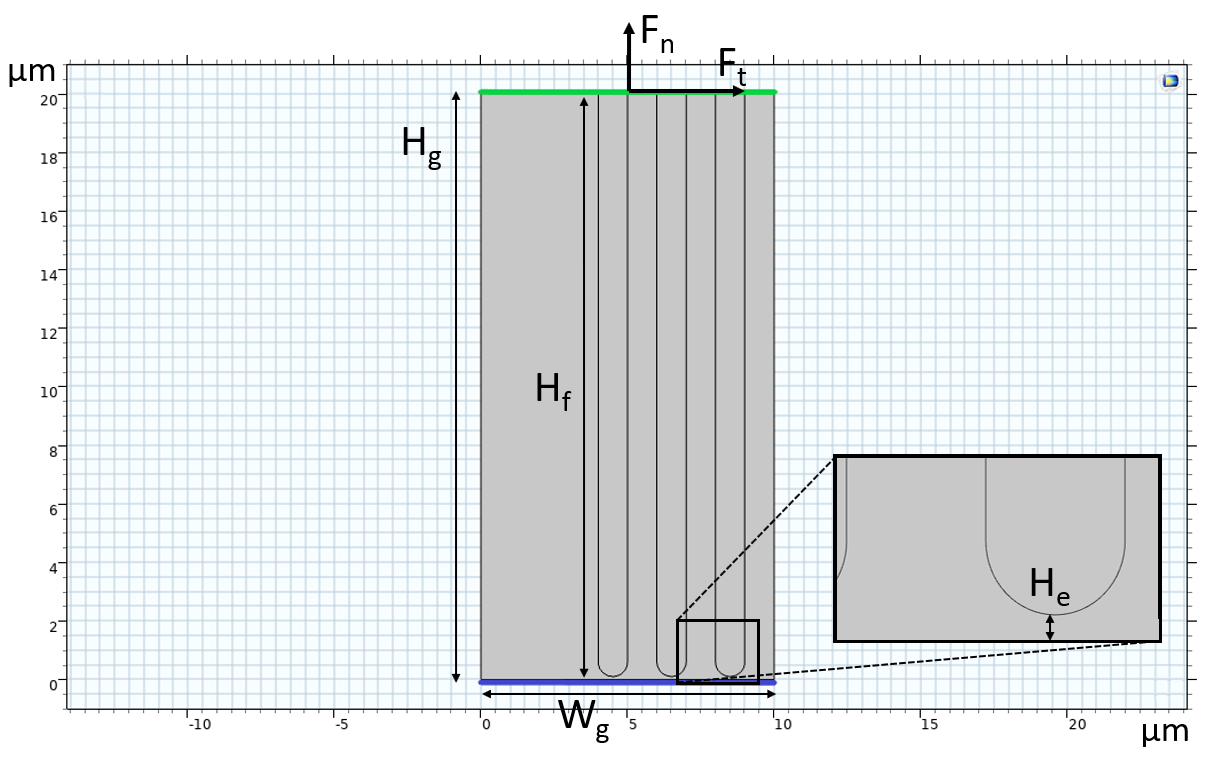
\includegraphics[width=0.8\linewidth, height=7.5cm, angle=0]{images/discrete_model_implementation/lever_distance.png}
    \caption{The dimensions involved in the boundary conditions of the simplified domain. The upper boundary is coloured green and is the point of application for the applied forces $F_n \& F_t$. The lower boundary is colored blue. The height and width of the domain are represented by $H_g \& W_s$ respectively. $H_f$ represent the length of the fibers and $H_e$ represent the distance between the fiber tips and the lower boundary.}
    \label{fig:boundary_conditions}
\end{figure}

\qquad The points of attention that to be addressed to obtain the required mechanical response for the simplified model with the rectangular domain are:
\begin{enumerate}
    \item The lower boundary of the domain is assumed fixed. This boundary condition can be applied since the contact with the substrate is assumed to be constant. The constant contact with the substrate also allows stress concentrations on the substrate do develop. This makes the mechanical behaviour more pronounced compared to a situation in which the lower boundary can adjust to applied loads. The geometry edges to which the boundary conditions are applied are visible in Figure \ref{fig:boundary_conditions}.
    \item Forces are applied on the upper boundary. This configuration resembles a situation in which the tree frog exerts a force on the substrate. This loading configuration is a simplification of the real situation in which the load would be more distributed over the domain. This is not considered an issue for a normal load $F_n$ since the flow direction of the stresses in the material is orthogonal to the upper boundary used for the load application in the simulation. A shear load $F_t$ however, induces a moment in the material which is dependent on the distance $H_g$ between the lower boundary and the plane of force application. This moment is less when the force is applied over the whole domain which shortens the length of the lever to $\frac{H_g}{2}$.
    \item The upper boundary is free in translation in the x and the y-direction but constrained in rotation. The rotational constraint is derived from the observation that the epithelial cells are concatenated and would therefore resist rotation of the upper boundaries. Fully constrained rotation is a simplified assumption of the real situation since the real situation would most probably offer a small amount of rotational freedom.
    \item The left and right sides of the geometry are left free. Although an epithelial cell is in constant contact with its surrounding cells on the sides, it can be assumed that all these cells are loaded in a similar way. This would result in a similar deformation pattern for neighbouring cells and with that no significant additional loads on the right and left boundaries of a simplified rectangular domain. 
    \item In Section \ref{sec:bio_material_properties} the stiffness of the individual epithelial cell components is discussed. These stiffness values are also used in the discrete fiber model. The influence of the variation of the stiffness for the different components is discussed in Section \ref{ch:results}.
    \item The simplified model uses a linear elastic material model for the fibers and the base material. This assumption is made after an evaluation of the differences between a hyperelastic and a linear elastic material model. The sensitivity of the simplified model is further evaluated in Section \ref{sec:discrete_model_sensitivities}.
    \item The length of the fibers $H_f$ and the size of the gap $H_e$ between the fiber tips and the substrate are kept constant for all the performed simulations. The thin layer ensures that the contact with the substrate is established with a continuous domain. This is a simplification of the real situation in which the contact is established with the thin cornified cell envelope which is also made visible in Figure \ref{fig:epithelial_cell_components}.
    \item The bonding between the fibers and the base material is assumed perfect in the simplified model which means that the stiffness of the bonding is equal to the stiffness of the most compliant material involved. The influence of this assumption and the impact of a change in the bonding between fibers and matrix is discussed in Sections \ref{sec:results_fiber_bonding} and \ref{sec:discrete_model_sensitivities}.
\end{enumerate}



\subsubsection{Model validation}\label{sec:discrete_model_validation}
Validation of the discrete fiber model is done by comparing the results of the discrete fiber model with the results obtained by Xue et al. \cite{xue2017hybrid}. These results are described in Section \ref{sec:tree_frog_applications}.\\

\qquad When a rectangular block of material uniform elastic or hyperelastic properties with a fixed base is loaded in tension, the stress concentrations are found at the corners of the geometry as is visible in Figure \ref{fig:uniform_elastic_stress}. The S22 stress component considered is equivalent to the S33 stress component considered by Xue et al. as visible in Figure \ref{fig:Xue_model_1} and \ref{fig:Xue_model_2}. The stiffness of the homogeneous material is set to $2 MPa$ with a Poison's ratio of $0.49$.\\

\begin{figure}[h!]
    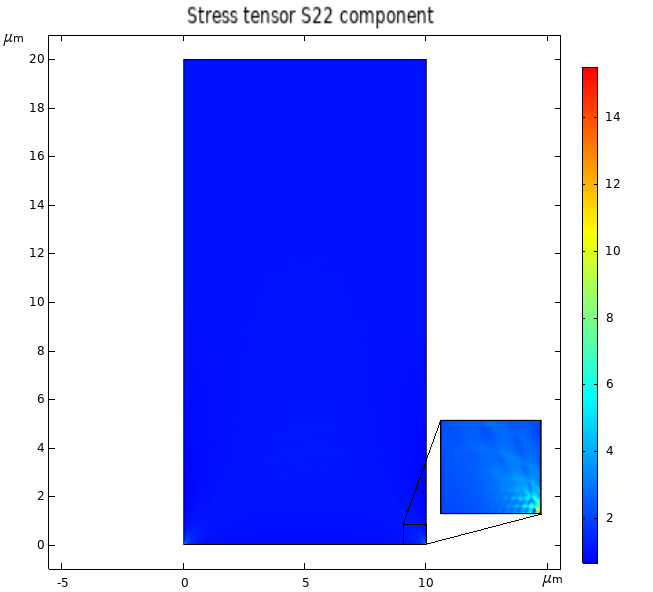
\includegraphics[width=0.7\linewidth, height=8.5cm, angle=0]{images/discrete_model_validation/blok_elastic.png}
    \caption{An uniform elastic domain with a fixed base loaded with a vertical load on the upper domain. The stress concentrations appear in the lower right and left corners. The stress concentration in the lower right corner is visible in the insert. The S22 component of the stress is considered.}
    \label{fig:uniform_elastic_stress}
\end{figure}

\qquad The stress distribution in the uniform domain can be compared with the stress distribution in a domain in which fibers are implemented. Figure \ref{fig:coarse_fibers} shows a domain in which coarse fibers are implemented. The stress is strongly influenced by the location of the fiber re-enforcement. The most important observation is that the fibre re-enforced model has a much lower value for the stress at the end of the geometry at $L = 10 \mu m$ on the horizontal axis. This reduction in peak stress increases the adhesive strength of the material since the stress are better divided over the contact interface compared to the uniform domain visible in Figure \ref{fig:uniform_elastic_stress}. The stiffness of the base material used for this model is $2 [MPa]$ and the stiffness of the fibers is set to $200 [MPa]$. A Poison's ratio of $0.49$ is implemented for the base material and the fibers.\\

\begin{figure}[h!]
    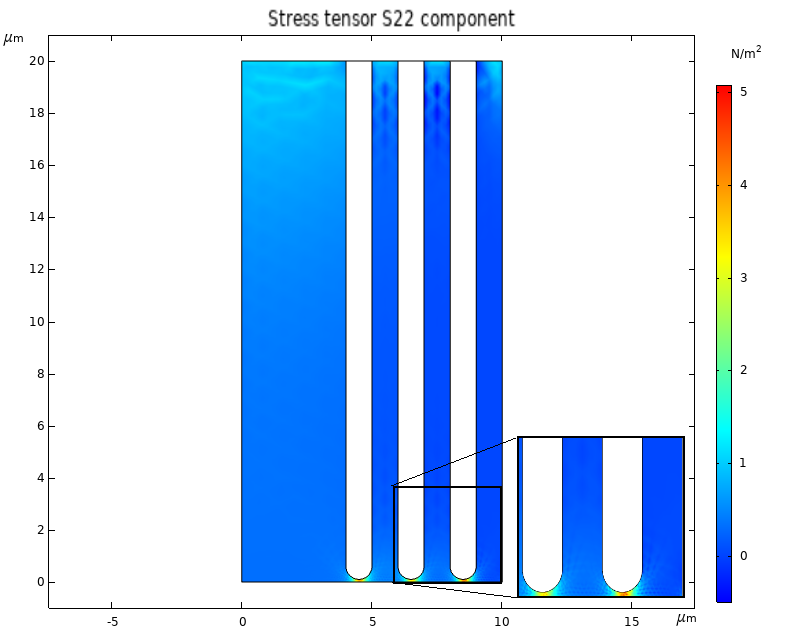
\includegraphics[width=0.7\linewidth, height=8.5cm, angle=0]{images/discrete_model_validation/coarse_fibers.png}
    \caption{A composite model with coarse fibers implemented in a relatively soft base material. The loading and boundary conditions of this model are similar to the model from Figure \ref{fig:uniform_elastic_stress}.}
    \label{fig:coarse_fibers}
\end{figure}

\qquad The stress concentrations visible in Figure \ref{fig:coarse_fibers} are very similar to what is visible in Figure \ref{fig:Xue_model_1}. In both models, a stress concentration occurs between the fibers and the contact surface. When the maximum of the stress magnitude is compared between Figure \ref{fig:uniform_elastic_stress} and Figure \ref{fig:coarse_fibers} it appears that the magnitude of the stress below the fibers in Figure \ref{fig:coarse_fibers} is significantly lower than the magnitude of the stress in the lower right corner of the geometry as visible in Figure \ref{fig:uniform_elastic_stress}. The maximum of the stress found in the composite material is a factor $\frac{15}{5} = 3$ lower than the maximum value of the stress in the continuous material domain.\\ 

\qquad These observations confirm that the stresses in the simplified composite model are indeed lower than the stresses in a geometry with homogeneous material properties. Furthermore, it is observed that the location of the maximum stress shifts from the corner of the geometry to a location under the fibers. These observations are also described by Xue et al. and validate the use of the simplified composite model.


\subsubsection{Model sensitivities}\label{sec:discrete_model_sensitivities}
This section describes the sensitivity of the discrete model to numerical effects and solver configurations. The sensitivity of the discrete fiber model to variation in model variables is described in Section \ref{sec:results_fiber_stiffness} and \ref{sec:results_fiber_bonding}.\\


% een sensitivity analysis generally describes the influence of a change in one of the model variables. The variables relevant for such a study in the case of the discrete model are:
%    - stiffness of the layer between the fibers and the base material
%    - Material model used for the base material
%    - Numerical instability due to the mesh density

% hier beschrijven

% hier ook de gevoeligheid voor ruis en meenemen, dit komt dan vervolgens weer terug in het gedeelte van de data processing

%  The adaptive mesh refinement algorithm will globally adjust the mesh to better resolve the local stresses, and these stresses depend on the solution everywhere else in the model. The solution smoothens out but takes to much mesh elements for the amount of memory available to fully smoothen out.(this partly works but is not the best option to come to a smooth solution)
%     https://www.comsol.com/blogs/using-adaptive-meshing-local-solution-improvement/
%     - smoothing is always an option...and is also done in the post-processing


\qquad The stress response of the model influenced numerical instability that is related to the mesh density and also known as the Runge's phenomenon. This phenomenon causes oscillation at the edges of an interval when a polynominal interpolation is used. This phenomenon can be countered by increasing the resolution of the mesh. This method increases the amount of mesh nodes. A more efficient way is a mesh refinement study that increases the mesh locally at the locations where steep gradients are encountered. The adaptive mesh algorithm does smooth the response but takes too much mesh elements for the available memory to compute a fully smooth model response.\\

\qquad Another way to smooth the response is an increase in the discretization order of the displacement field. Increasing the discretization order also increases the memory needed for the computation and causes memory errors when the discretization order is too large. An increase in the discretization order however, significantly smooths out the solution as is visible in Figure \ref{fig:discretization_order}.\\

\begin{figure}[h!]
    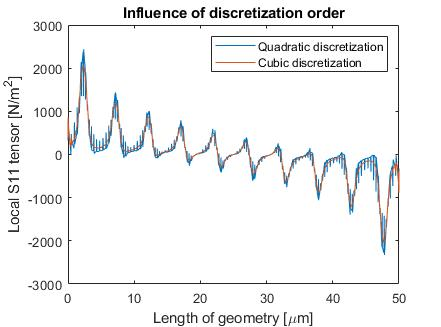
\includegraphics[width=0.65\linewidth, height=7cm, angle=0]{images/discrete_model_sensitivities/Influence_discretization_order.jpg}
    \caption{Model stress response for different discretization orders. The cubic discretization gives a smoother response than the quadratic discretization but is more computational demanding.}
    \label{fig:discretization_order}
\end{figure}

\qquad The discrete fiber model that uses linear elastic material properties does encounter non-linear behaviour is certain loading configurations. This is the case when a shear and a normal load are simultaneously applied. This non-linear behaviour can lead to convergence issues. To prevent these and to shorten computation time the estimates of the initial values of the dependent values need to be chosen carefully. Comsol Multiphysics uses these values as an estimate for the computational result and therefore benefits from an accurate prediction of these values.\\ 
    
    

\subsubsection{Data processing}\label{sec:discrete_model_data}
% hier beschrijven hoe je de data uit het comsol model heb gekregen en hoe je deze data daarna verwerkt hebt in Matlab. Dit kan allemaal kort en bondig!

The stresses of the discrete fiber model are evaluated at the lower boundary of the geometry. The values of the stress components are evaluated in a cut line which is defined just above the lower geometry boundary at $y = 0.001 \mu m$. The $S_{11}$ and $S_{22}$ stress components are extracted from the Comsol simulation.\\ 

\qquad The discretization order of the displacement field in the Comsol model is set to quadratic. In Section, it was discussed that this discretization can be increased to produce a smoother stress response. This however significantly increases the computational demands of the model. The discretization order of the model is therefore not increased and the results are smoothed out using a moving average in the post-processing of the results. This produces similar results compared to the results that are produced with a higher discretization order.\\


\subsection{HGO model}\label{sec:HGO_model}
The HGO model allows the implementation of of directional dependent properties in a model. This allows the implementation composite material properties in a continuous domain. This reduces the amount of mess elements needed for the implementation of composite material properties.

\subsubsection{Model fundamentals}\label{sec:HGO_model_fundamentals}
The formulation of the possible linear material transformations for an orthotropic material is visible in Equation \ref{eq:general_transformation} which shows the stress vector $\sigma$, the strain vector $\epsilon$ and the fourth order stiffness tensor $C$ \cite{freutel2014finite}. The material properties of an orthotropic material are different along the orthogonal axis of the material.\\ 

\begin{gather}
    \sigma = C \epsilon,\nonumber\\[1ex]
    \text{With for $\sigma$, $\epsilon$ and $C$:}\nonumber\\[1ex]
    \sigma  = \begin{bmatrix}
    \sigma_{11}\\
    \sigma_{22}\\
    \sigma_{33}\\
    \sigma_{23}\\
    \sigma_{13}\\
    \sigma_{12} \end{bmatrix},\quad
    \epsilon = \begin{bmatrix}
    \epsilon_{11}\\
    \epsilon_{22}\\
    \epsilon_{33}\\
    2 \epsilon_{23}\\
    2 \epsilon_{13}\\
    2 \epsilon_{12} \end{bmatrix},\nonumber\\
    C = \begin{bmatrix}
    C_{1111} & C_{1122} & C_{1133} & 0 & 0 & 0\\
    C_{2211} & C_{2222} & C_{2233} & 0 & 0 & 0\\
    C_{3311} & C_{3322} & C_{3333} & 0 & 0 & 0\\
    0 & 0 & 0 & C_{2323} & 0 & 0 \\
    0 & 0 & 0 & 0 & C_{1313} & 0 \\
    0 & 0 & 0 & 0 & 0 & C_{1212} \end{bmatrix},\nonumber\\[1ex]
    \text{With}\nonumber\\[1ex]
    C_{2211} = C_{1122}, C_{3311} = C_{1133}, C_{3322} = C_{2233}
    \label{eq:general_transformation}
\end{gather}

\qquad Biological materials often have similar properties in two orthogonal directions. This is caused by the (local) orientation of the fibers in these biological materials. The modifications needed to represent such a transversal isotropic material by the fourth order stiffness tensor $C$ from Equation \ref{eq:general_transformation} are visible in Equation \ref{eq:mod_stiffness_tensor} \cite{freutel2014finite}.

\begin{gather}
    C_{2211} = C_{1122}, C_{3311} = C_{1133} = C_{3322} = C_{2233},\nonumber\\
    C_{1111} = C_{2222},\nonumber\\
    C_{2323} = C_{1313},\nonumber\\
    C_{1212} = \frac{1}{2}(C_{1111} - C_{1122})
    \label{eq:mod_stiffness_tensor}
\end{gather}

\qquad These equations allow the implementation of direction-dependent material properties but represent only linear material deformations. The fibres in biological materials however, often display non-linear material behaviour. Fibres are often much stiffer in tension than in compression \cite{li2009three} and can also display strain-dependent elastic properties. Hyperelastic material properties can be described with several material models. Examples of such models are the neo-Hookean material model \cite{ogden1997non} and the Mooney–Rivlin model \cite{mooney1940theory}.\\

\qquad In order to model the non-linear properties of the materials present in the epithelial cell of the tree frog, a material model is needed that describes material behaviour of the fibers and the ground substance in which the fibres are embedded. The fiber orientation in the keratinous domain of the epithelial cell is a function of the location which makes the material properties direction and location dependent.\\

\qquad The HGO model introduced by Holzapfel et al.\cite{holzapfel2000new} can be used to implement the directional and location dependent material behaviour. This model allows modelling of composite fibrous materials with anisotropic hyperelastic properties. These hyperelastic properties can be implemented for both the ground substance and for the embedded fibers. The equations for the HGO model describe the isochoric strain energy density which is defined as visible in Equation \ref{eq:isochoric_strain_energy}. The parameter $W_{1}$ describes the contribution of the material in which the fibres are embedded and $W_{4}$ describes the contribution of the fibres. Both parameters are derived using Equation \ref{eq:F} - \ref{eq:elastic_cauchy_green_tensor}. 
  
\begin{equation}
      W_s = W_{1} + W_{4}
      \label{eq:isochoric_strain_energy}
\end{equation}

\qquad In order to construct the parameters $W_1$ and $W_4$, it is required to go back to some basic relations. The deformation of a material can be described with the deformation gradient $\textbf{F}$ given in Equation \ref{eq:F}. This gradient is composed of a parameter describing the rotation $\textbf{R}$ and of a parameter which describes the translation from the undeformed to the deformed composition $\textbf{V}$. The left Cauchy-Green deformation tensor $\textbf{B}$ can be constructed from the deformation gradient $\textbf{F}$ and is visible in Equation \ref{eq:B}. These basic equations can be used to construct the invariant $\overline{\textbf{I}}_{1}$ which is used to describe the incompressible material behaviour as visible in Equation \ref{eq:invariant_incompressible_mat}. This invariant uses the jacobian $\textbf{J}$ of $\textbf{F}$ and the invariant $\textbf{I}_{1}$ with is defined as $\textbf{I}_{1} = tr(\textbf{B})$.

\begin{equation}
    \textbf{F} = \textbf{V} \textbf{R} 
    \label{eq:F}
\end{equation}

\begin{equation}
    \textbf{B} = \textbf{F} \textbf{F}^T = \textbf{V}^2
    \label{eq:B}
\end{equation}

\begin{equation}
    \overline{\textbf{I}}_{1} = \textbf{J}^{- \frac{2}{3}} \textbf{I}_{1}
    \label{eq:invariant_incompressible_mat}
\end{equation}

\qquad The invariant $\textbf{I}_4$ is dependent on the direction of the fibres and on the local deformation gradient. Equations \ref{eq:I4_short} and \ref{eq:I4_long} show the short and the long notation of the invariant respectively. The invariant is composed of a vector field $\textbf{a}$ which represents the direction of the fibres and the isochoric elastic Cauchy-Green tensor $\overline{C_{el}}$.

\begin{equation}
    I_{4} = \textbf{a} \overline{\textbf{C}_{el}} \textbf{a}
    \label{eq:I4_short}
\end{equation}
  
\begin{equation}\label{eq:I4_long}
  \begin{split}
       I_{4} & = a_{1} \overline{C_{el_{11}}} a_{1} 
            + 2a_{1} \overline{C_{el_{12}}} a_{2}
            + 2 a_{1} \overline{C_{el_{13}}} a_{3}\\
            & + a_{2} \overline{C_{el_{22}}} a_{2}
            + 2 a_{2} \overline{C_{el_{23}}} a_{3}
            + a_{3} \overline{C_{el_{33}}} a_{3}
        \end{split}
 \end{equation}
 
 \qquad The isochoric elastic Cauchy-Green tensor $\overline{\textbf{C}_{el}}$ as visible in Equation \ref{eq:elastic_cauchy_green_tensor} is constructed from the local elastic Cauchy-Green tensor $\textbf{C}_{el_{ij}}$ and from the elastic volume ratio $\textbf{J}_{el}$. Subscripts $i$ and $j$ express the local coordinates. $\textbf{C}_{el_{ij}}$ is constructed from the inverse of the inelastic deformation gradient and from the local Cauchy-Green tensor. This local Cauchy-Green tensor is constructed from the local deformation gradients as visible in Equation \ref{eq:local_cauchy-green_tensor}. This equation sums over $n$ dimensions and uses the deformations in the $i$ and in the $j$ directions.

\begin{equation}
    C_{l_{ij}} = \sum_{n=1}^{3} F_{ni} F_{nj}
    \label{eq:local_cauchy-green_tensor}
\end{equation}

\begin{equation}
    \overline{\textbf{C}_{el}}_{_{ij}} = \textbf{J}^{-\frac{2}{3}}_{el} \textbf{C}_{el_{ij}}
    \label{eq:elastic_cauchy_green_tensor}
\end{equation}
  
 \qquad The parameters $\overline{I}_{1}$ and $I_{4}$ can now be used to define the parameters from Equation \ref{eq:isochoric_strain_energy}. $W_1$ is the isotropic function with describes the isotropic behaviour of the material in which the fibres are embedded. This function depends on one material parameter $C_{10}$ and the first invariant of isochoric elastic right Cauchy-Green tensor $\overline{I}_{1}$ as visible in Equation \ref{eq:first_isochoric invariant}. The parameter $W_4$ represents the contribution of the anisotropic material properties. As visible in Equation \ref{eq:anisotropic_w4}, $W_4$ is dependent on the parameters $k_1$ and $k_2$ which respectively represent a stress like material parameter and a dimensionless constant. The invariant $I_4$ is  visible in Equation \ref{eq:I4_long}. The parameter $k_{2}$ represents the amount of non-linearity in the material. This parameter gives the amount of strain stiffening.
  
 \begin{equation}
      W_1 = \frac{C_{10}}{2}(\overline{I_{1}}) - 3)
      \label{eq:first_isochoric invariant}
 \end{equation}
  
\begin{equation}
    W_4 = \frac{k_1}{2k_2}(e^{k_2(I_4 - 1)^2} - 1)
    \label{eq:anisotropic_w4}
\end{equation}

\subsubsection{Model implementation: geometry}\label{sec:HGO_model_geometry}
The working principle of the keratinous structure, is not expected to be dependent on an exact number of fibres. The most important characteristic of the fibrous structure is that of an anisotropic material. Furthermore, it is expected to display non-linear material behaviour. The HGO material model (see section about modelling methods) allows the implementation of anisotropic hyperelastic materials. With this approach, the material properties of the keratinous fibres are dependent on a location dependent vector field. The streamlines of this vector field are visible in Figure \ref{fig:streamlines}.\\ 

\begin{figure}[h!]
    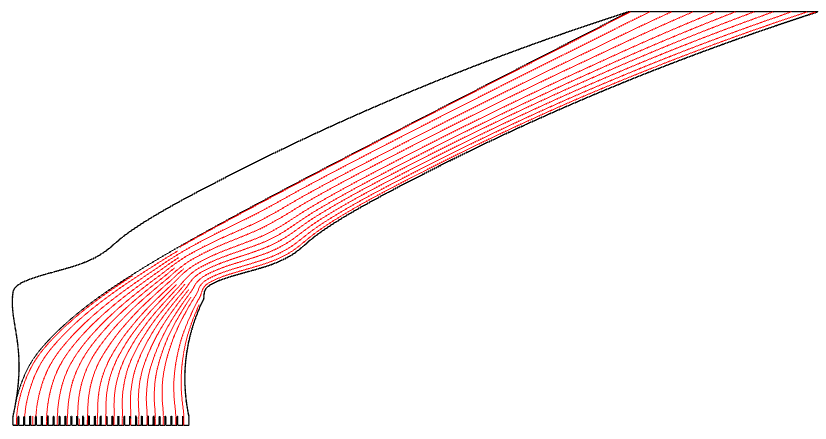
\includegraphics[width=0.55\linewidth, height=5cm, angle=0]{images/HGO_model_geometry/geometry_streamlines.PNG}
    \caption{The outer contours of the epithelial cell with the streamlines that indicate the direction of the keratinous fibers.}
    \label{fig:streamlines}
\end{figure}

\qquad The working principle of the HGO model is also implemented in a simplified square domain. This domain is similar in dimensions as for the models visible in Figure \ref{fig:uniform_elastic_stress}. 





\subsubsection{Model implementation: boundary conditions}\label{sec:HGO_boundary_conditions}
The HGO model is implemented in both the simplified rectangular domain and in the geometry which resembles the epithelial cell. The boundary conditions of the simplified rectangular domain can be found in Section \ref{sec:discrete_model_boundary_con}. The boundary conditions for the geometry resembling the epithelial cell are described in this section and visible in Figure \ref{fig:BC_HGO_model}.\\ 
% These are to some extent equal to the boundary conditions implemented for the simplified geometry with the discrete fibers. 

% beschreven voor het discrete fiber model:
% - Op welke grenzen er welke krachten werken
% - de stijfheid van de individuele componenten
% - geometrische parameters: afstanden tussen fibers en celgrens
% - bonding tussen fibers en matrix materiaal


\begin{figure}[h!]
    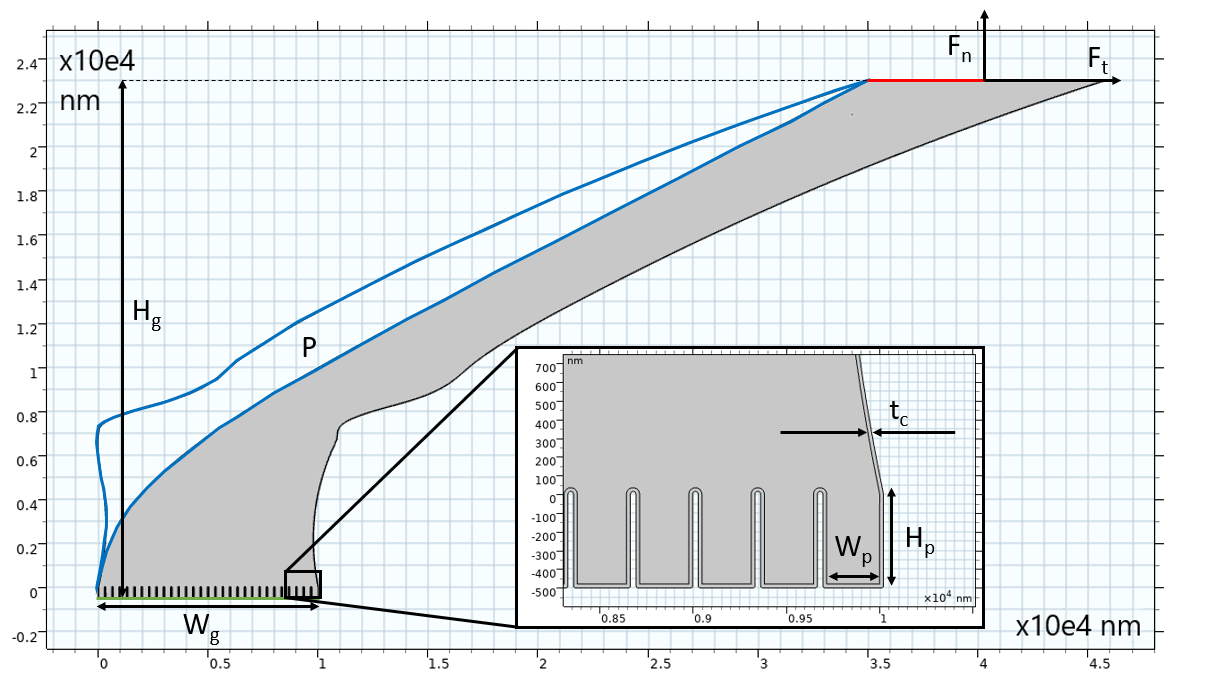
\includegraphics[width=0.9\linewidth, height=8cm, angle=0]{images/HGO_model_geometry/BC_HGO_model.png}
    \caption{The dimensions and boundary conditions of the model which resembles the epithelial cell. The lower boundary is coloured green, the upper boundary is coloured red. The lower boundary is fixed while the external forces $F_{n} \& F_{t}$ are applied on the upper boundary. The blue boundaries enclose the lymph space. The lymph fluid exerts a pressure $P$ on the boundaries of the lymph space. $H_{g}$ and $W_g$ represent the height and base width of the epithelial cell respectively. The epithelial cell is enclosed by a cornified cell layer with thickness $t_{c}$. The epithelial cell has a total of 30 pillars. The height and width of these pillars is represented by $H_{p}$ and $W_{p}$ respectively.}
    \label{fig:BC_HGO_model}
\end{figure}

\qquad The points of attention to be addressed to obtain a mechanical response that matches best with the mechanical behaviour of a real epithelial cell are:
\begin{enumerate}
    \item The lower geometry boundary, highlighted in green in Figure \ref{fig:BC_HGO_model} is fixed. This assumption is also implemented in the simplified rectangular geometry described in Section \ref{sec:discrete_model_boundary_con}. The reasons for the implementation of this condition are the same for the epithelial cell based geometry. % fixed bottom
    \item The upper boundary is loaded with the applied forces $F_{n} \& F_{t}$ these forces resemble the  the perpendicular and tangential loads respectively. This loading configuration is a simplification of the real loading configuration in which the loads would be more evenly distributed over the material domain. % loads on the upper boundary
    \item The boundary conditions on the left and right cell boundaries are necessary to prevent unrealistic deformations in the y-direction. The relatively large distance in the x-direction between the point of application of the forces and the point of application of the reaction force on the base of the epithelial cell can cause a large deformation in the y-direction when a normal force is applied. In reality however, the space under the epithelial cell is filled with other cells which will resist such a large deformation. To resemble the mechanics of the neighbouring cells, the lower boundary is subjected by a force per unit area in the x and y-direction. These parameters are represented by $\sigma_{xx}$ and $\sigma_{yy}$ which are defined as visible in Equation \ref{eq:BC_right}. In these equations the displacement is represented by $u$ and $v$. The parameter $L$ represents an estimate of the maximum displacement and the parameter $E_s$ represents the Young's modulus of the surrounding cellular material. The values of these parameters is $10 \mu m$ and $100 kPa$ respectively. The value of $E_s$ is derived from the indentation experiments performed by Barnes et al. as can be seen in Table \ref{tab:experiments_literature}. % The left and right boundaries
    
    \begin{gather}
        \sigma_{xx} = \frac{-u}{L} E_{s},\nonumber\\
        \sigma_{yy} = \frac{-v}{L} E_{s}
        \label{eq:BC_right}
    \end{gather}
    
    \item The upper boundary of the cell (in red in Figure \ref{fig:BC_HGO_model}) is constrained in rotation. This condition resembles a realistic situation in which concatenated cells will not have full rotational freedom. This condition is also described in Section \ref{sec:discrete_model_boundary_con}. % rigid connector on the upper boundary
    \item The lymph fluid in the domain enclosed by the boundaries visible in blue in Figure \ref{fig:BC_HGO_model} consists mainly out of water which can be assumed an incompressible fluid. Equation \ref{eq:BC_pressure} defines the pressure $P$ on the boundaries of the lymph space as a function of the initial undeformed area $A_{0}$ and the variable area $A$ of the domain. This is a simple and effective way of maintaining a constant volume in an enclosed domain. The surface area of the lymph domain is defined with an integration on the domain borders. The displacement of the lymph fluid is considered irrelevant and therefore excluded. This also saves computational resources. 
    
    \begin{equation}
         P = A - A_{0}
        \label{eq:BC_pressure}
    \end{equation}
    % pressure in the cytoplasm
    \item The mechanical properties implemented for the cornified cellular layer are based on a the assumption that this relatively thin layer(10 nm) has linear elastic properties with a Young's modulus of $100 [MPa]$, a Poisson ratio of $0.4$ and a density of $1000 [kg/m^3]$. These properties bring the mechanical behaviour in the range of other keratinous bio-materials as discussed in Section \ref{sec:bio_material_properties}.   % the properties of the cornified cellular layer
    \item The mechanical properties of the fibrous domain are implemented with the HGO model. This material model requires the constants $k_1$ and $k_2$ which are both associated with the anisotropic contribution of the fibres to the overall response. The stiffness of the fibers is expressed by $k_1$ and $k_2$ represents the amount of fiber non-linearity. This non-linear behaviour is visible in the amount of strain stiffening since the fibres in the implemented model to not have any stiffness in compression. The material stiffness of the base material is represented by the parameter $C_{10}$. Based on the stiffness values described in Section \ref{sec:bio_material_properties}, the true stiffness of the connective tissue is expected to fall in a range of $C_{10} = 1-10 [MPa]$ and the stiffness of the keratin is expected to be the range of $K_1 = 1-10 [GPa]$. Typical values for the parameter $k_2$ are between 0.5 and 5. The first approximation implemented in the model is $k_{2} = 1$. The value of the parameter $k_1$ is varied, this is discussed further in Section \ref{sec:results}.\\ % HGO model constants
\end{enumerate}






\subsubsection{Model validation}\label{sec:HGO_model_validation}
% de validadtie voor het discrete model is als volgt:
% - vergelijking van een blok met linear elastische eigenschappen 
% - met een blok met composiete materiaal eigenschappen
% - dit wort dan weer vergeleken met het model van xue et al.

% in dit gedeelte een geometrie met dunne fibers die dan beter in de buurt moet komen van het HGO model en het HGO model zelf
The HGO model is basically a simplified version of a fiber re-enforced material in which the fibers are relatively thin and everywhere present such that the directional properties of the fibers are present everywhere in the material. For validation of the HGO material model, this model can be compared with the model of Xue et al. as is also described in Section \ref{sec:discrete_model_validation}. 


\begin{figure}[h!]
    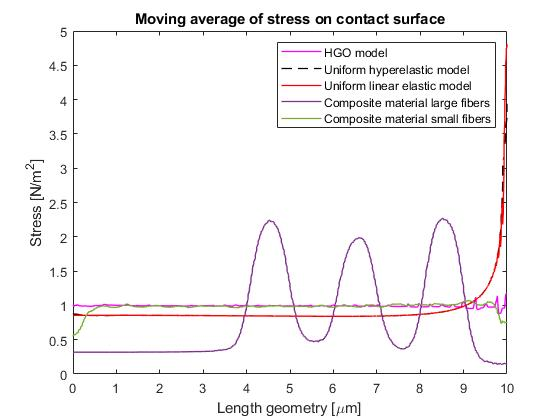
\includegraphics[width=0.6\linewidth, height=6cm, angle=0]{images/HGO_model_validation/validatie_matlab_plot.jpg}
    \caption{The $S_{22}$ component of the stress along the length of the geometry for different material models. The models are all loaded with an equal force in the y-direction while the loer boundary of is fixed. The stress response of the uniform linear elastic model and the uniform hyperelastic model are very similar and are added for comparison with the composite material models and the HGO model.}
    \label{fig:HGO_validation}
\end{figure}

The validation of the HGO model is divided in several steps in which the fiber density is increased from a few discrete fibers with finite thickness to an infinite number of infinitely thin fibers. The $S_{22}$ component of the stress response of the different models is visible in Figure \ref{fig:HGO_validation}. 
\begin{enumerate}
    \item The first step of the validation involves the discrete fiber model discussed in Section \ref{sec:discrete_model_validation}. This model involves only a few and relatively thick discrete fibers which are well bounded to the matrix material. The largest magnitude of the stress is visible between the fibers and the contact surface.
    \item The second step in the validation of the HGO model involves a model in which more and thinner fibers are present. In this model is visible that the stress concentrations are still visible at the tips of the fibers. The magnitude of the stress at the tips of the fibers however, is much lower compared to the stresses visible for the coarse fiber model. The mechanical behaviour of the fine fiber model shows that a finer fiber configuration is beneficial for the magnitude of the contact stresses. The stress drops at the edge of the geometry where no fibers are located. 
    \item Based on the stress distribution of the fine fiber model, the stress distribution of the HGO model can be expected to be uniform over the whole length of the domain since the mechanical properties of the fibers are present everywhere in the geometry. The stress response of the HGO model as visible in Figure \ref{fig:HGO_validation} does meet this expectation. This model is set up
    with the parameters $k_{1} = 2 [MPa]$ and $k_{2} = 200 [MPa]$. The difference between the fine fiber model and the HGO is also visible in Figure \ref{fig:HGO_fine_fibers_val}. The largest difference between these two models is visible near the boundary of the geometry. This is mainly caused by the absence of fibers near the boundary of the geometry for the fine fiber model. The peaks of the HGO model near the right edge of the boundary are caused by numerical instability and will be further discussed in Section \ref{sec:HGO_model_sensitivities}. 
\end{enumerate}

\begin{figure}[h!]
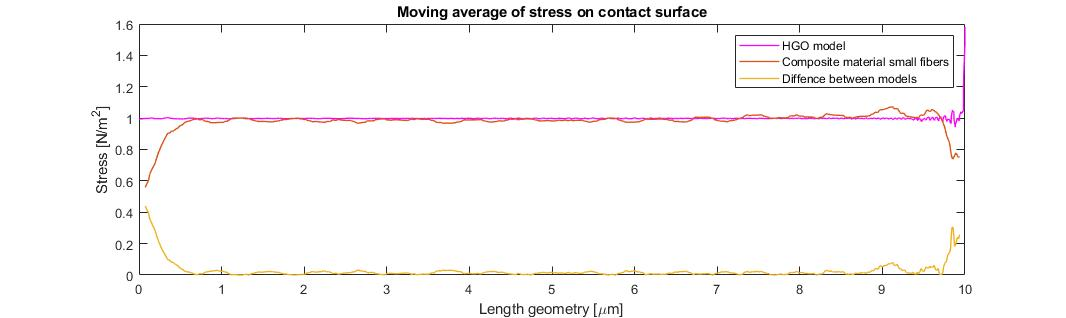
\includegraphics[width=0.6\linewidth, height=3.5cm, angle=0]{images/HGO_model_validation/validatie_HGO_en_fine_fibers.jpg}
\caption{Difference between the HGO model and the fine fiber model.}
\label{fig:HGO_fine_fibers_val}
\end{figure}

% nog even over de validatie, is het goed genoeg?
\qquad The modelling results discussed above validate the use of the HGO model for a geometry which would otherwise be filled with fine fibers. The validation described above however, only validates the HGO model for a configuration in which the load is applied in the direction of the fibers. Therefore, this validation needs to be elaborated to investigate the validity of the HGO model for a case in which the geometry is not loaded in the direction of the fibers.\\


\qquad Figure \ref{fig:HGO_validation_1} shows the $S_{22}$ stress component in an simplified geometry that is loaded with a force in the x-direction(perpendicular to the direction of the fibers) and with a force in the y-direction. The stress values of the models loaded in tension are comparable with the stress values visible in Figure \ref{fig:HGO_validation}. The model results of the models loaded with a normal and a shearing force show that a shearing force significantly increases the stress in the geometry. This increase in stress is also visible for the $S_{11}$ stress component. The $S_{13}$ component is zero along the whole length of the lower geometry boundary. Figure \ref{fig:HGO_validation_1} shows the stress in the lower left corner of the geometry while the same effects in the stress response can also be observed in the lower right corner.\\  

\begin{figure}[h!]
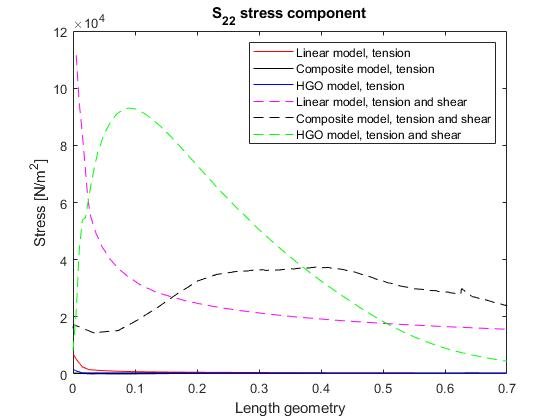
\includegraphics[width=0.7\linewidth, height=6.5cm, angle=0]{images/HGO_model_validation/comparison_all_data.jpg}
\caption{Stress response of the linear model, the fine fiber and the HGO model for different loading configurations.}
\label{fig:HGO_validation_1}
\end{figure}

\qquad The difference between the stress distribution for the HGO model and the composite model increases with the introduction of the shear force. When loading a geometry like the geometry visible in Figure \ref{fig:uniform_elastic_stress} with a force in the x-direction while the bottom is fixed, a bending moment is created. This bending moment introduces reaction forces in the y-direction from which the magnitude and forces are dependent on the location in the geometry. These reaction forces are the largest at the right and left boundaries of the geometry. This is also visible in the $S_{11}$ and $S_{22}$ stress components which are the largest near the lower right and left corners of the geometry. The forces in the x-direction are the sum of the shear forces and the forces induced via the deformations caused by the forces in the y-direction. This second component is dependent on the constant value of the Poison ratio.\\ 


\qquad Figure \ref{fig:HGO_validation_2} shows the these stress components for a rectangular geometry with the same dimensions as visible in Figure \ref{fig:uniform_elastic_stress}. This geometry is fixed at the lower boundary and the right boundary is loaded with a force in the x-direction. In these figures it is visible that:

\begin{enumerate}
    \item In the right subplot of Figure \ref{fig:HGO_shear_S22} is visible that the $S_{22}$ component for the HGO model when loaded in compression and in shear is very similar to this component for the linear model. This can be explained by the absence of directional dependent properties for the HGO model when loaded in compression. Without these directional dependent properties, the HGO model acts as a pure solid with a Neo-hookean material model. The stress response of a solid geometry with a Neo-hookean material model is very similar to the response of a linear elastic material model for the boundary and loading conditions used in this validation simulation.
    \item In the left subplot of \ref{fig:HGO_shear_S22} is visible that the different variations of the HGO model do have a stress peak in the left corner of the geometry. This stress peak is most probably caused by the strain stiffening properties of the HGO model. This effect can be expected at the left corner of the geometry due to the reaction forces implied by the imposed moment which are in the direction of the strain stiffening material model properties.  
    \item The $S_{11}$ component visible in the corners of the geometry visible in both subplots of Figure \ref{fig:HGO_shear_S11} follows the deformation that is caused by the $S_{22}$ component. The deformation at the very left edge is relatively low due to the strain stiffening effect discussed above. This is most probable the reasons why the peak of the $S_{11}$ component occurs right before the left edge of the geometry as visible in the left subplot of Figure \ref{fig:HGO_shear_S11}. 
    \item The stress components of the linear composite model in the left corner of the geometry visible in the left subplots of Figure \ref{fig:HGO_shear_S11} \& \ref{fig:HGO_shear_S22} are much lower than the stresses found for the other material models. The main reasons for this is most probable caused by the buffering nature of the complient material situated at the edge of the geometry for the discrete fiber model geometry. The strain at the edges of the linear composite model is visible in Figure \ref{fig:i4_invariant}. This invariant can be calculated with Equation \ref{eq:I4_short} and represents the strain in the direction of the fibers. In Figure \ref{fig:i4_invariant} is visible that the linear composite model has more strain at the edges than the HGO model. This strain however, does not result in a higher values for the $S_{11}$ and $S_{22}$ stress components because of the buffering nature of the outer compliant layer present at the edge of the composite linear model. The relatively low strain for the HGO model can be explained with the strain stiffening effect. 
    \item The strain stiffening composite model is similar to the linear composite model but has fibers that display non-linear strain stiffening behaviour. This strain stiffening behaviour is also discussed for other bio-materials \cite{holzapfel2000new}. The mechanical properties of these fibers are similar to these of the HGO model with $C = e$ used in Equation \ref{eq:w4_var}. The $S_{11}$ and $S_{22}$ components found for the strain stiffening composite model display that the strain stiffening leads to a higher stress at the top of the fibers as visible in the left subplots of Figure \ref{fig:HGO_shear_S11} \& \ref{fig:HGO_shear_S22}. The directional dependence of the strain stiffening properties however, leads to higher values for the $S_{11}$ and $S_{22}$ components in the right corner of the geometry as visible in the right subplots of Figure \ref{fig:HGO_shear_S11} \& \ref{fig:HGO_shear_S22}. It is visible for this model that the buffering nature of the complient layer at the left edge of geometry prevents the development of stresses. This effect is also described for the linear composite model, but on both edges. 
\end{enumerate}


\begin{figure}[h!]
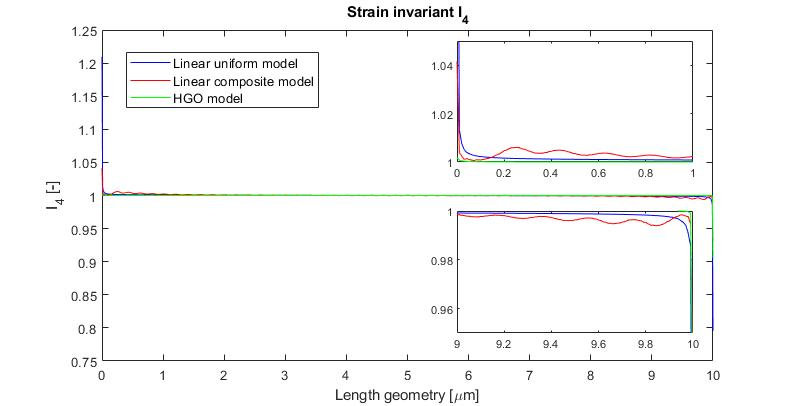
\includegraphics[width=0.7\linewidth, height=6.5cm, angle=0]{images/HGO_model_validation/Invariant_i4.jpg}
\caption{Strain invariant for different material models. The invariant has a value of one for zero strain conditions.}
\label{fig:i4_invariant}
\end{figure}


% nog goed naar het composite lineare model kijken!
%  - wat als het composite model niet lineaire eigenschappen heeft?
%  - geen significante verandering voor niet lineare eigenschappen van het composiet lineare model


%hier nog verder gaan over de strain stiffening properties 
\qquad The $S_{11}$ and $S_{22}$ stress components visible in Figure \ref{fig:HGO_shear_S11} \& \ref{fig:HGO_shear_S22} are plotted for three variants of the HGO model to provide insight in the strain stiffening properties of the HGO model. The strain stiffening behaviour of this model is determined by Equation \ref{eq:anisotropic_w4}. This equation can also be written as visible in Equation \ref{eq:w4_var}. The effects of varying the parameter $C$ are visible in Figure \ref{fig:HGO_shear_S11} \& \ref{fig:HGO_shear_S22}. As is visible in this figure, the stress in the x-direction can be brought closer to the response of the fibrous model by tuning the exponential function that determines the $W_{4}$ component of the HGO model.\\ 

\begin{equation}
    W_4 = \frac{k_1}{2k_2}(C^{k_2(I_4 - 1)^2} - 1)(I_{4}>1)
    \label{eq:w4_var}
\end{equation}

\qquad The reduction of the peak magnitude of the $S_{11}$ component is most probably caused by the decreased strain at the locations where the strain stiffening occurs. The $S_{22}$ component of the stress in these locations does not match the response of the fibrous model. The slope of this component however, is affected by the tuning of the parameter $C$ as visible in left subplot of Figure \ref{fig:HGO_shear_S22}.\\

\qquad The tuning of the $W_{4}$ component of the HGO model gives the best results for the default value $e$ for the parameter $C$. Values higher or lower than $e$ give a worse result in therms of the stress peak visible in the left subplot of Figure \ref{fig:HGO_shear_S11}. The maximum value of the $S_{22}$ component visible in the left and right subplot of Figure \ref{fig:HGO_shear_S22} is the lowest for the smallest value for $C$. This can be explained by the reduced effect of the strain stiffening for this value. The magnitude of $C$ therefore determines the ratio of the $S_{11}$ and $S_{22}$ components.\\ 

\begin{figure}[h!]
    \begin{subfigure}{0.95\textwidth}
    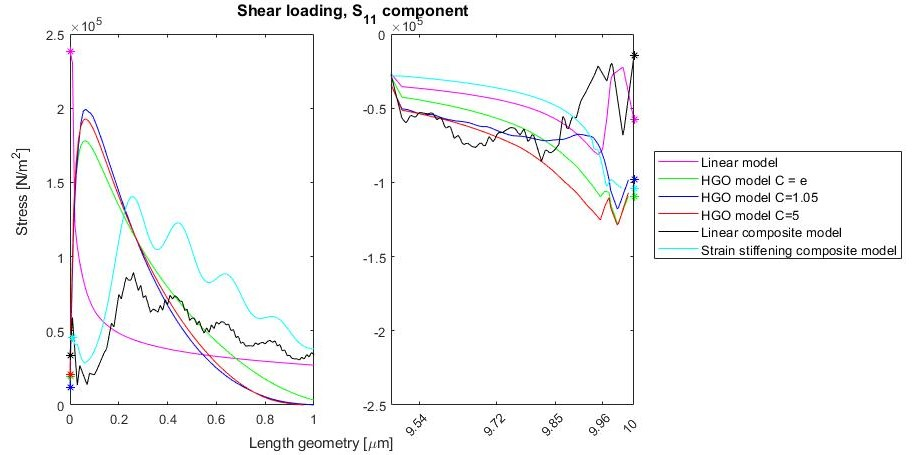
\includegraphics[width=\textwidth, height=7cm, angle=0]{images/HGO_model_validation/HGO_model_shear_S11.jpg}
    \caption{}
    \label{fig:HGO_shear_S11}
    \end{subfigure}
    \hfill
    \begin{subfigure}{0.95\textwidth}
    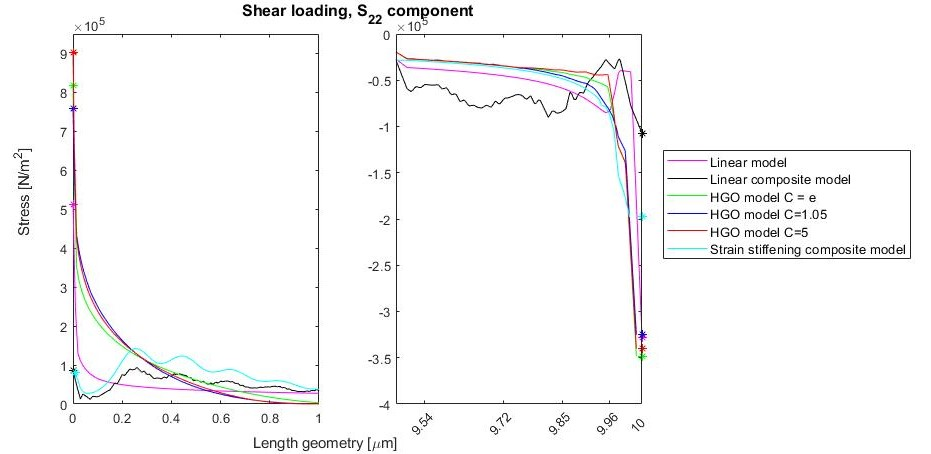
\includegraphics[width=\textwidth, height=7cm, angle=0]{images/HGO_model_validation/HGO_model_shear_S22.jpg}
    \caption{}
    \label{fig:HGO_shear_S22}
    \end{subfigure}
    \caption{The $S_{11}$ and $S_{22}$ stress components in the x-direction and y-direction for a shear loaded configuration of the simplified HGO model. The asterisks at the start and the end of the curves mark the value of the stress components at the outer edges of the geometry.}
    \label{fig:HGO_validation_2}
\end{figure}

\qquad The observations in this section point out that the HGO model differs from the discrete fiber model when the load on the geometry causes a non-uniform distribution of forces along the interface between the geometry and the substrate. This is caused by the strain stiffening of the HGO model and the buffering nature of the compliant material present along the edges of the composite material model.\\ 

\qquad Modelling a complex geometry with a large number of mesh elements as is visible in Figure \ref{fig:geometry_solidworks} requires a material model in which individual fibers are not present. The HGO model meets this requirement. This model however does differ from the (strain stiffening) composite model as discussed above. These differences are taken into account when discussing the modelling results of the model that incorporates the geometry visible in Figure \ref{fig:geometry_solidworks}.\\




% hier redenen bedenken..kan het het nog dichterbij gebracht worden en kan de sensitivity analysis hier bij helpen?





\subsubsection{Model sensitivities}\label{sec:HGO_model_sensitivities}
% In order to tune the HGO model as good as possible to the expected material properties of the tree frog, the parameters $c_10$, $k_1$ and $k_2$ are varied to evaluate their influence on the HGO model behaviour. The HGO model is again implemented for a rectangular domain with the same dimensions as used for the validation step and the forces and boundary conditions applied are the same as described for Figure \ref{fig:test_geometry}.\\ 

% Variations of the parameter $k_2$ while the other parameter are kept constant do not change the stresses in the material. The parameter $k_2$ does only effect the strain stiffening behaviour of the model. therefore, it only effects the amount of deformation of the model, in particular the strain of the geometry caused by the $S_{22}$ component of the stress. 

% The parameters the stiffness of the base material and fibrous component is described by respectively $c_M$ and $k_1$. The influence of the value of these two parameters is investigated by varying these parameters with respect to each other by varying $k_1$ while keeping $c_M$ at a constant value. The value of $k_1$ is given by the relation $k_1 = c_M R$ with $R$ representing the ratio between $c_M$ and $k_1$. The deformation and stress for $R = 100$ are visible in Figure \ref{fig:tuning_deformation}. In this figure is visible that the highest stresses occur at the lower left corner of the geometry. 

% \begin{figure}[h!]
%     \includegraphics[width=\linewidth, height=6cm, angle=0]{Pictures/tuning/deformation.png}
%     \caption{Deformation of the domain and visualization of the $S_{22}$ stress component.}
%     \label{fig:tuning_deformation}
% \end{figure}

% Figure \ref{fig:tuning_11_com} and \ref{fig:tuning_22_com} show that the $S_{11}$ and the $S_{22}$ components are both influenced bu the value of the parameter $R$. For high values of $R$ the stress in the lower left corner of the geometry reaches significantly higher values than for lower values for this parameter. 

% \begin{figure}[h!]
%     \centering
%   \subfloat[\label{fig:tuning_11_com}]{%
%       \includegraphics[width=\linewidth, height=6.5cm, angle=0]{Pictures/tuning/stress_11_var_cmk1.jpg}}
%     \hfill
%   \subfloat[\label{fig:tuning_22_com}]{%
%         \includegraphics[width=\linewidth, height=6.5cm, angle=0]{Pictures/tuning/stress_22_var_cmk1.jpg}}
%   \caption{Stress component $S_{11}$ and $S_{22}$ for various values of the ratio between the HGO model parameters $c_M$ and $k_1$. The x-axis has a logarithmic scale to visualize the stress at the left edge of the geometry.}
% \end{figure}
% \subsubsection{Solver configuration}
%  the model involves non-linear behaviour which can sometimes lead to convergence issues. The measures taken to prevent convergnece issues and to shorten computation time are as follows:
%  - the estimates of the initial values of the dependent values need to be chosen carefully. Comsol uses these values as an estimate for the computional result and therefore benefits from an accurate prediction of these values. 
 
%   % question:
%  % why is the model more computational intensive for a larger ratio between Cm and k1?
%  Although the properties of the HGO model are already compared with the model using by Xue et al., it still makes sense to investigate if the introduction of a shear force force does effect the model performance. Figure \ref{fig:validation_shear} shows the absolute value of an average stress in the geometry when this geometry is loaded with both shear and a perpendicular load. This average value is composed of the stress components $S_{11}$ and $S_{22}$ represented by Equation \ref{eq:average_stress}. The $S_{13}$ component is zero along the whole length of the lower geometry boundary and is therefore not taken into account. The stress values represented with the continuous lines are comparable with the values visible in Figure \ref{fig:HGO_and_fine_fibers} while the dotted lines represent the model results for a model which also includes a shearing force. This additional shearing force significantly increases the stress in the geometry. The difference between the stress distribution for the HGO model and the composite model increases with the introduction of the shear force. This can be caused by...% hier redenen bedenken..kan het het nog dichterbij gebracht worden en kan de sensitivity analysis hier bij helpen?
 
 
 
 
 
 
\subsubsection{Data processing}




\section{Experimental setup}


\begin{table}[h!]
    \centering
    \begin{tabular}{|l|c|c|c|}\hline
    \diaghead{\theadfont Diag ColumnmnHead}%
    {Stiffness PDMS}{Fiber thickness}&
    \thead{Reference,\\no inserted fibers} & \thead{Thin fibers} & \thead{Coarse fibers}\\ 
    \hline
    $1 [MPa]$ & I & II & III \\    
    \hline
    $3 [MPa]$ & IV & V & VI \\    
    \hline
    \end{tabular}
    \caption{Different test pieces fabricated}
    \label{tab:experimental_variants}
\end{table}


\subsection{Modelling}
% het tweede orde ogden model is gevonden als het beste om hyperelastisch materiaalgedrag van PDMS te modelleren. De parameters zijn gefit in het artikel van Kim et al. \cite{kim2011measurement}
  
%   de parameter zijn $\mu_1 = 63.49$ [MPa] en $\mu_2 = 0.041$ [MPa] met $\alpha_1 = 	6.371e-10$ en $\alpha_2 = 3.81166$ en een bulk modulus van $962$ [MPa] voor een mengverhouding van basis polymeer en curing agent van 1:10. The density of PDMS is $965 [kg/m^3]$.
  
  
%   het tweede orde ogden model is gevonden als het beste om hyperelastisch materiaalgedrag van PDMS te modelleren. De parameters zijn gefit in het artikel van Kim et al. \cite{kim2011measurement}
% de parameter zijn $\mu_1 = 63.49$ [MPa] en $\mu_2 = 0.041$ [MPa] met $\alpha_1 = 	6.371e-10$ en $\alpha_2 = 3.81166$ en een bulk modulus van $962$ [MPa] voor een mengverhouding van basis polymeer en curing agent van 1:10. The density of PDMS is $965 [kg/m^3]$.
\subsection{Fabrication}
\subsection{measurement setup}
\subsection{Boundary conditions}
\subsection{Data processing}